\documentclass[10pt,fleqn,xcolor=dvipsnames]{beamer}
\beamertemplatenavigationsymbolsempty
\usetheme{Boadilla}
\DeclareGraphicsExtensions{.jpg,.eps,.png,.pdf,.mps,.gif}
\usepackage[latin1]{inputenc}
\usepackage[T1]{fontenc}
\usepackage[english]{babel}
\usepackage{pgf,pgfarrows,pgfnodes,pgfautomata,pgfheaps}
\usepackage{amsmath}
\usepackage{amsfonts}
\usepackage{graphicx}
\usepackage{color}
\usepackage{lmodern}
\usepackage[3D]{movie15}
\usepackage{algorithm}
\usepackage{algpseudocode}
\usepackage{url}
\usepackage{placeins}
\usepackage{textcmds}
\usepackage{listings}

\colorlet{grey}{gray!40}
\definecolor{PG}{rgb}{0.0, 0.27, 0.13}
%%%%%%%%%%%%%%%%%%%%%%%%%%%%%%%%%%%%%%%%%%%%%%%%%%%%%%%%%%%%%%%%%%%%%%%%%%%%%%%%%%%%%%%
% title page definition %%%%%%%%%%%%%%%%%%%%%%%%%%%%%%%%%%%%%%%%%%%%%%%%%%%%%%%%%%%%%%%
%%%%%%%%%%%%%%%%%%%%%%%%%%%%%%%%%%%%%%%%%%%%%%%%%%%%%%%%%%%%%%%%%%%%%%%%%%%%%%%%%%%%%%%
\setbeamercovered{dynamic}
\setbeamerfont{author}{family=\rmfamily}
\author[M. Beccuti,   R. J. P. Bonnal
and  R. Calogero]{\large{\textbf{M. Beccuti,  R. J. P. Bonnal
 and R. Calogero}}\\[15pt]\emph{Universit\`{a} degli Studi di Torino \\  Istituto Nazionale di Genetica Molecolare \qq{Romeo ed Enrica Invernizzi}
}\\~\\~ \textbf{ELIXIR-IIB Training Platform}~\\\tiny(First day)}
\title[Docker and Reproducibility]{\Large{\textbf{Docker and Reproducibility}}}
%\institute{\normalsize{} \\
%\footnotesize{Boston Park Plaza Hotel, Boston, Massachusetts USA}}
\date[June 2019]{June 2019}
\titlegraphic{
\begin{flushright}

\includegraphics[height=2cm]{Figure/LogoTorino}
\includegraphics[height=2cm]{Figure/LogoINGM_original}
\end{flushright}
}

% table of contents depth
\setcounter{tocdepth}{1}
\begin{document}
\usebackgroundtemplate{
\includegraphics[width=140mm]{Figure/BackgroundTorino}}
\setcounter{tocdepth}{5}
%#Frame 1 title
\frame[plain]{\titlepage}


\frame{
  \frametitle{Outline}  \vspace{0.3cm}
    \begin{block}{Training aims:}
\begin{itemize}
\item Create and run  a docker image; 
\item Develop a  docker service;
\end{itemize}    
\end{block}
}
\frame{
\frametitle{Outline} \vspace{0.3cm}
 \vspace{0.5cm}
\begin{enumerate}
\item Introduction\vspace{0.2cm}
\begin{itemize}
\item Virtualization: Virtual Machines and containers; \vspace{0.2cm}
\item Containers in Linux: Docker project; \vspace{0.2cm}
\end{itemize}
\item Command Line Interface
\item A simple example: how to embed an application in a Docker Image; \vspace{0.2cm}
\begin{itemize}
\item DockerHub
\item Volumes: sharing data with the containers
\item Building a Docker image with R
\end{itemize}
\item dockerfile \vspace{0.2cm}
\begin{itemize}
\item scripting the build of an Image
\item building a custom Image using a dockerfile
\item dockerfile best practices
\end{itemize}
\end{enumerate}
  }


 \frame{
  \frametitle {}
  \vspace{2cm}
  \centerline{\Huge \color{NavyBlue} \textbf{\emph{Introduction}}}
  \vspace{0.5cm}
     	\begin{center}
  			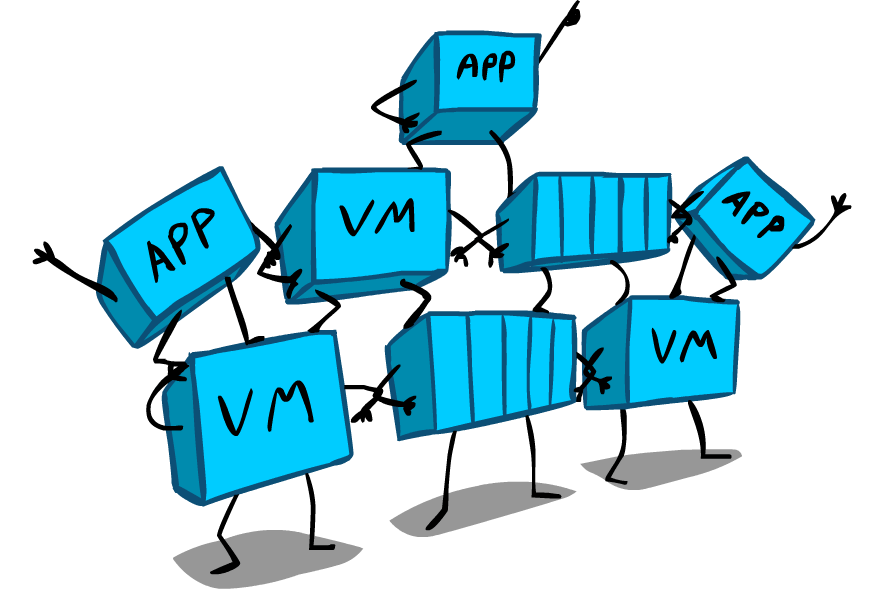
\includegraphics[width=0.50\columnwidth]{./Figure/VMDOC}
  		\end{center} 
}


 \frame{
  \frametitle{In the dark ages...}
         	\begin{center}
  			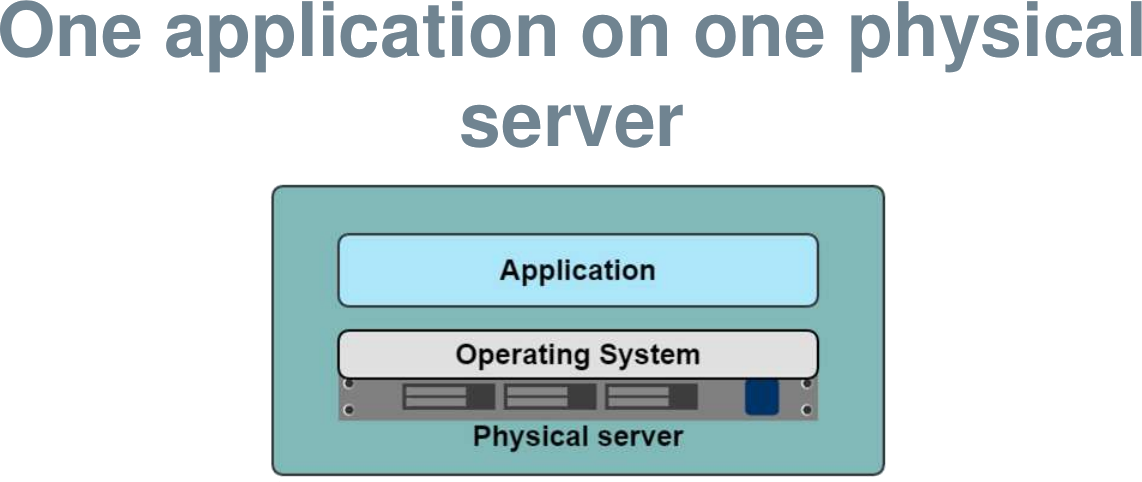
\includegraphics[width=0.80\columnwidth]{./Figure/singleapp}\\
  		\end{center} 
   \begin{columns}[T] % align columns		
   \begin{column}{.40\textwidth}   				
   \begin{itemize}
  		\item Wasted resources;
  		\item Difficult to migrate;
  		\item Difficult to scale;  
  \end{itemize}
\end{column}%
   \hfill%
   \begin{column}{0.35\textwidth}
      \begin{itemize}
     	\item Slow deployment rate;
  	 	\item Huge costs.
      \end{itemize}
   \end{column}%
   \end{columns}

  } 
  
  \frame{
  \frametitle{Virtual machines (VM)  and containers provide}  \vspace{0.25cm}  
 \begin{itemize}
 \item Better resource utilization:\vspace{0.15cm}
	\centerline{\color{NavyBlue}\emph{Multiple  VMs/containers can run on the same physical machine}}\vspace{0.2cm}
 \item Better service scalability:\vspace{0.15cm}
 \centerline{\color{NavyBlue}\emph{New VMs/containers associated with a service can be started when needed}}\vspace{0.2cm}
 \item Better level of portability and adaptability:\vspace{0.15cm}
  \centerline{\color{NavyBlue}\emph{VMs/containers can easily migrate from a server to another}}\vspace{0.2cm}
  \item Higher reproducibility level:\vspace{0.15cm}
    \centerline{\color{NavyBlue}\emph{Using VMs/containers we can freeze the version of tools, libraries ...}}
\end{itemize}\vspace{-0.15cm}
\begin{center}
  			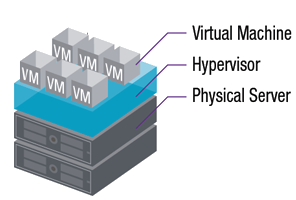
\includegraphics[width=0.35\columnwidth]{./Figure/vm3}~~~~
  			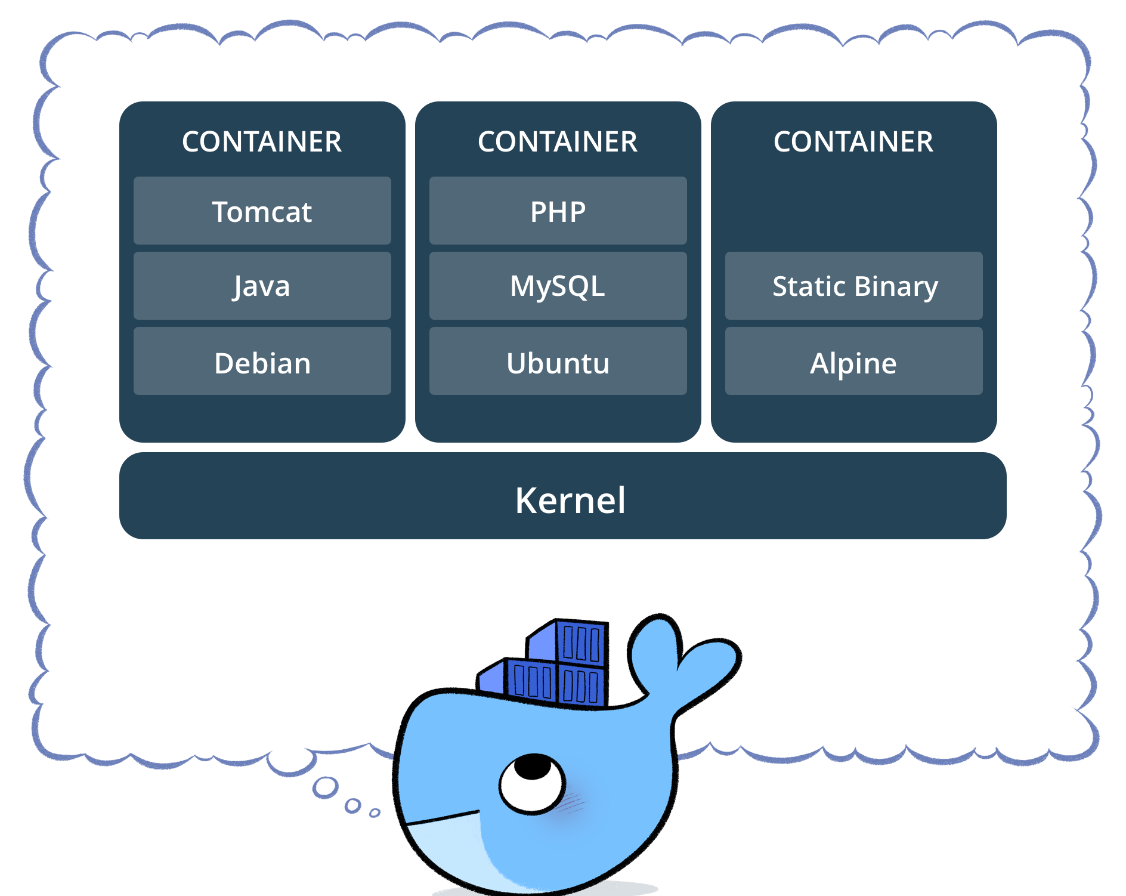
\includegraphics[width=0.27\columnwidth]{./Figure/dockerGen}
  		\end{center} 
}
  
  
  
  
 \frame{
  \frametitle {Containers VS Virtual Machines}
 % \vspace{0.3cm}
  % \textbf{\color{NavyBlue}Containers VS VM}\vspace{-0.5cm}
  \begin{columns}[T] % align columns
  \begin{column}{.50\textwidth}
  \vspace{0.8cm}
		\begin{center}
  			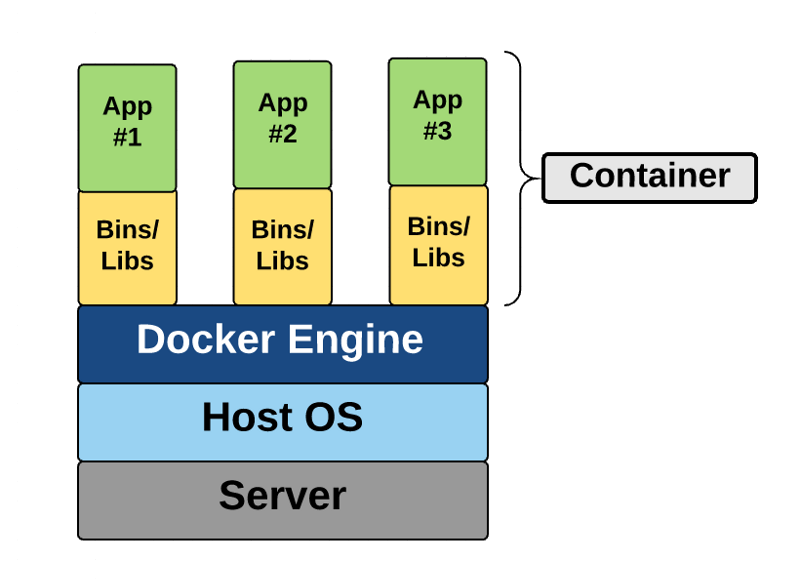
\includegraphics[width=1.00\columnwidth]{./Figure/Container}\\
  		\end{center}\vspace{-0.4cm}
  		Containers are an application level construct.
   \end{column}%
   \hfill%
   \begin{column}{0.50\textwidth}
     	\begin{center}
  			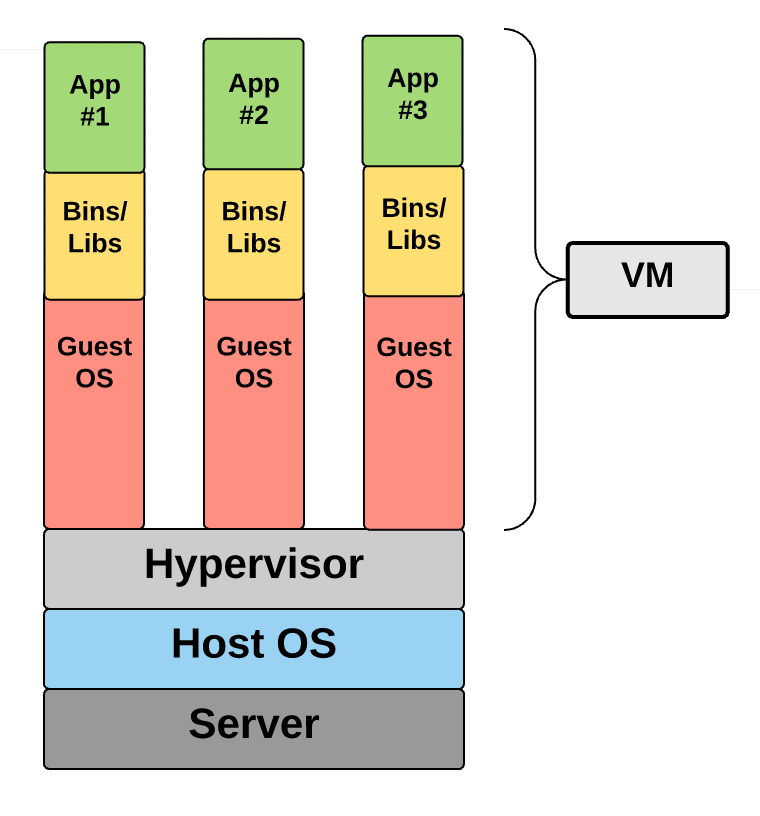
\includegraphics[width=1.00\columnwidth]{./Figure/vm2}\\
  		\end{center}
  	\vspace{-0.4cm}VMs are an infrastructure level construct. 
   \end{column}%
   \end{columns}
  }   
  
  
  
  \frame{
  \frametitle {Containers VS Virtual Machines}
 	\begin{center}
  			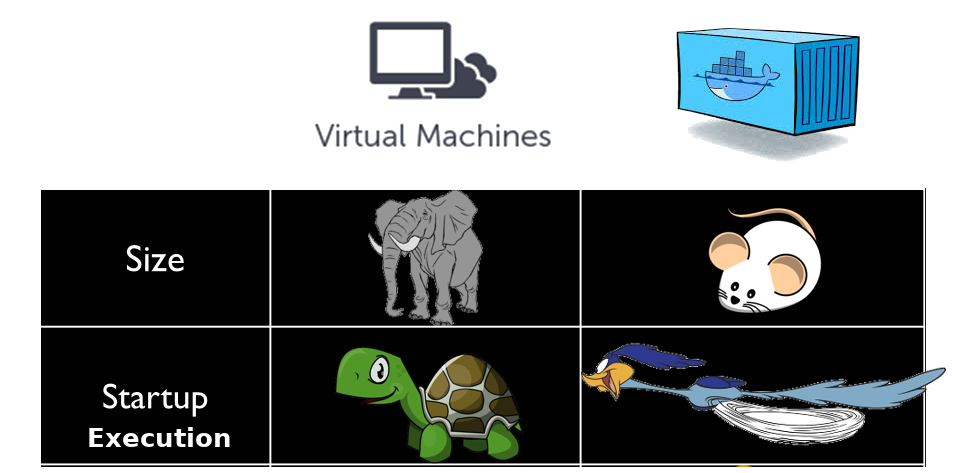
\includegraphics[width=0.90\columnwidth]{./Figure/ContainersVSVM}\\
  		\end{center}
  		
  \textbf{\color{NavyBlue}\emph{In Containers the sharing of the same OS Kernel with the real machine reduces the application portability, but ....}	}	
  } 


\frame{
\frametitle{Container, VM and real server: a comparison}
In [1] a comparison among physical server, KVM, and Docker is reported.

     	\begin{center}
  			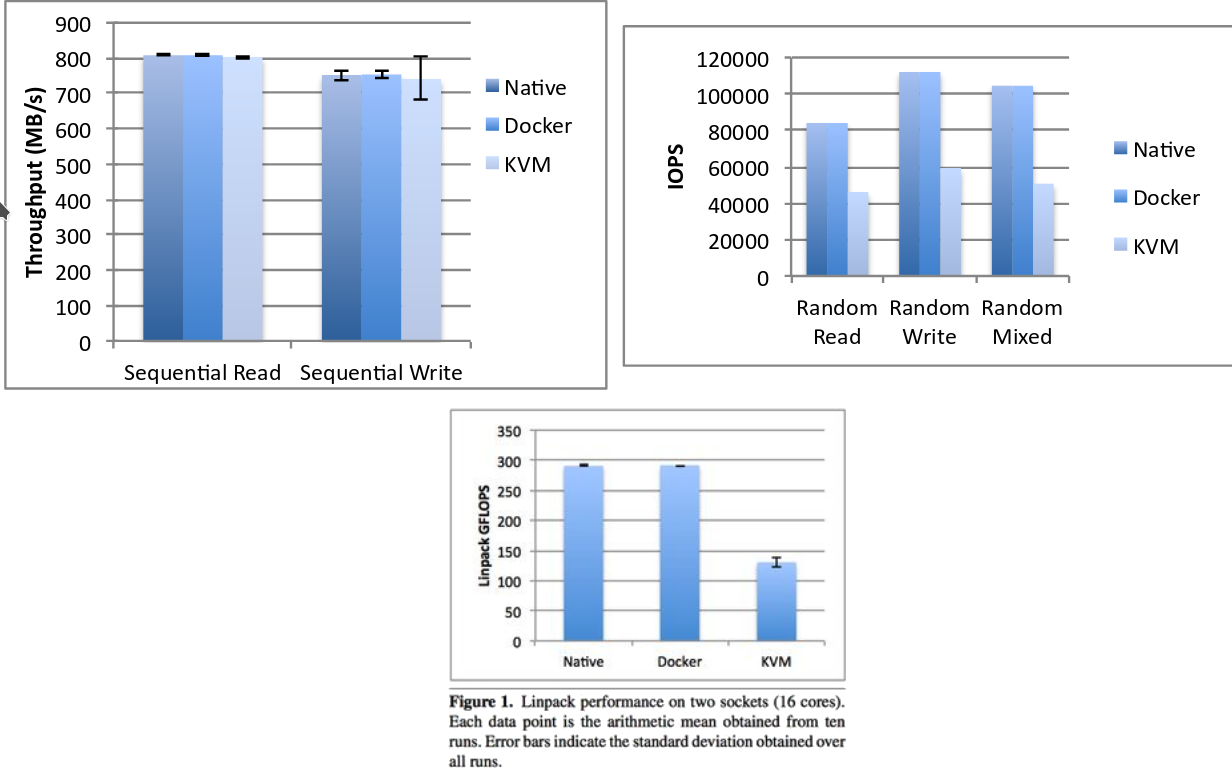
\includegraphics[width=0.90\columnwidth]{./Figure/benchmark}
  		\end{center}  
{\tiny
[1] W. Felter, A. Ferreira, R. Rajamony and J. Rubio, \emph{\textbf{An updated performance comparison of virtual machines and Linux containers}}, 2015 IEEE International Symposium on Performance Analysis of Systems and Software (ISPASS), Philadelphia, PA, 2015, pp. 171-172.

}
} 

  
  
\frame{
  \frametitle {Docker project}
  
  
  
  \begin{columns}[T] % align columns
  \begin{column}{.55\textwidth}
  	\begin{itemize}
 		\item Docker is an open-source project based on Linux containers.
 	\vspace{0.3cm}
 		\item Others Linux container technologies include Solaris Zones, BSD jails, and LXC, which have been around for many years.
 		 	\vspace{0.3cm}	
      	\end{itemize}
   \end{column}%
   \hfill%
   \begin{column}{0.45\textwidth}
   \vspace{-1.2cm}
     	\begin{center}
  			
\includegraphics[width=1.05\columnwidth]{./Figure/Docker}\\
  		\end{center}
   \end{column}%
   \end{columns}
   \vspace{0.8cm}
   \centerline{\Huge \color{NavyBlue} \textbf{\emph{Why to choose Docker?}}}
  } 
  
\frame{
  \frametitle {Why to use Docker?}
  
    \begin{columns}[T] % align columns
  \begin{column}{.65\textwidth}
  	\begin{itemize}
	\item  \textbf{\color{NavyBlue} Ease of use:} Docker has made it much easier for anyone to take advantage of containers in order to quickly build and test portable applications; \vspace{0.3cm}	
	
	\item  \textbf{\color{NavyBlue} Speed:} Docker containers are very lightweight and fast.
	\vspace{0.3cm}	
	\item \textbf{\color{NavyBlue}Docker Hub:} Docker users also benefit from the increasingly rich repository of Docker Hub, which you can think of as an ``app store for Docker images''; 
	\vspace{0.3cm}	
	\item \textbf{\color{NavyBlue}Modularity and Scalability:} Docker makes it easy to break out your application's functionality into individual containers.
  	\end{itemize}
   \end{column}%
   \hfill%
   \begin{column}{0.35\textwidth}
     	\begin{center}
  			
\includegraphics[width=1.05\columnwidth]{./Figure/Docker}\\
  		\end{center}
   \end{column}%
   \end{columns}
  } 
    


  \frame{
  \frametitle{Docker family picture} \vspace{0.3cm}
  \begin{center}
  			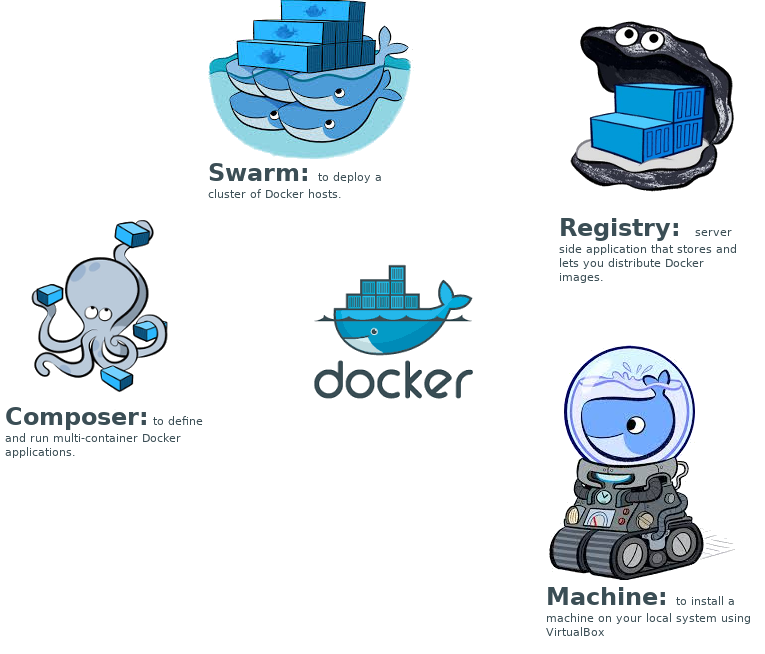
\includegraphics[width=0.77\columnwidth]{./Figure/family2}\\
  		\end{center} 
 } 	

 		
\frame{
\frametitle{Docker basics} 
\vspace{0.2cm}
\begin{itemize}
\item \textbf{\color{NavyBlue}\emph{Image}} is an executable package that includes everything needed to run an application (i.e. its code,  libraries, environment variables, and configuration files);\vspace{0.2cm}
\item \textbf{\color{NavyBlue}\emph{Container}} is a run-time instance of an image;\vspace{0.2cm}
\item \textbf{\color{NavyBlue}\emph{Volume}} is used to  share files from the host machine to containers.
\end{itemize}
\vspace{0.2cm}
  \begin{center}
  			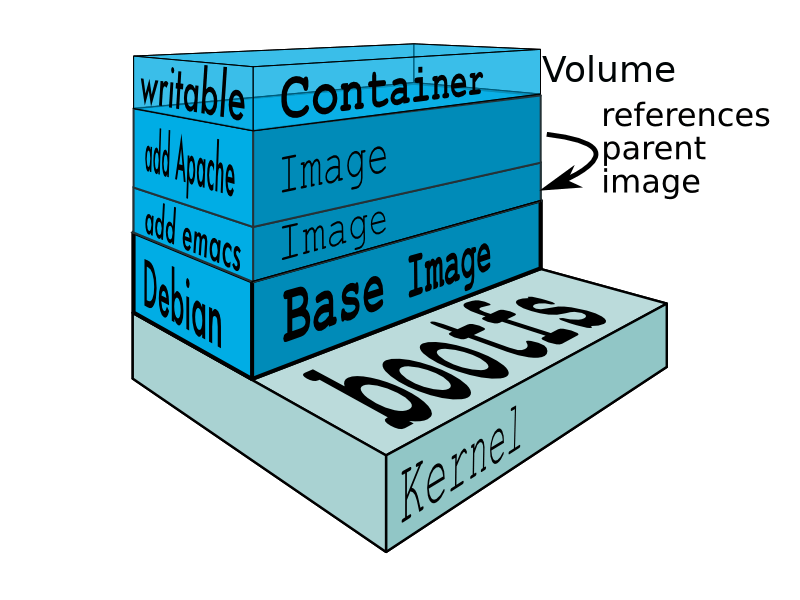
\includegraphics[width=0.55\columnwidth]{./Figure/exec}\\
  		\end{center} 

}

\frame{
\frametitle{Docker architecture} 
  \begin{center}
  			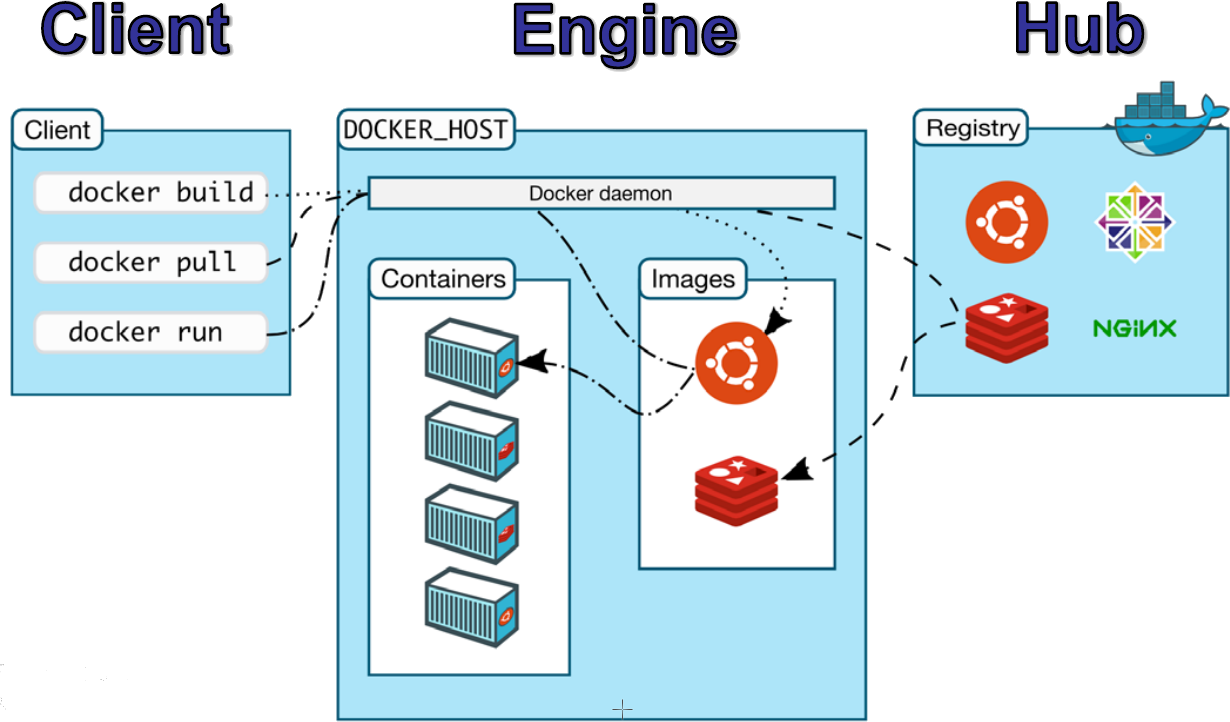
\includegraphics[width=1.02\columnwidth]{./Figure/arc}\\
  		\end{center} 

} 	
 
 \frame{
\frametitle{Docker client} 
    \begin{columns}[T] % align columns
  \begin{column}{.65\textwidth}
  \vspace{2.5cm}
  	\begin{itemize}
	\item It provides  an interface for users;\vspace{0.3cm}	
	\item It is cross Platform:  OSX,  Windows and  Linux;\vspace{0.3cm}	
	\item It allows  Local and Remote Execution.\vspace{0.3cm}	
  	\end{itemize}
   \end{column}%
   \hfill%
   \begin{column}{0.35\textwidth}
     	\begin{center}
  			
\includegraphics[width=1.00\columnwidth]{./Figure/Client}
  		\end{center}
   \end{column}%
   \end{columns}
  } 
  
   \frame{
\frametitle{Docker engine} 
    \begin{columns}[T] % align columns
  \begin{column}{.65\textwidth}
  \vspace{0.5cm}
  	\begin{itemize}
	\item It executes the commands received by the Docker Client;\vspace{0.3cm}
	\item It builds and menages images;	\vspace{0.3cm}	
	\item It creates and menages the Containers.\vspace{0.3cm}	
  	\end{itemize}
   \end{column}%
   \hfill%
   \begin{column}{0.38\textwidth}
     	\begin{center}
  			
\includegraphics[width=1.00\columnwidth]{./Figure/engine}
  		\end{center}
   \end{column}%
   \end{columns}
  } 
  
  
\begin{frame}
\frametitle{Goals}
\begin{itemize}
\item  using docker to deploy an application
\item  also in HPC setting
\item  different use cases:
  \begin{itemize}
    \item  single application, temporary container
    \item  complex application, temporary container
    \item  lightweight Virtual Machine, always-on container
    \end{itemize}
\end{itemize}
\end{frame}

\begin{frame}
\frametitle{Container - Reproducibility}
\begin{itemize}
\item  Reuse existing images with a precise version of OS and software
\begin{itemize}
   \item   Docker facilitates this integrating the concept of \qq{reuse if possible} in its core
\end{itemize}
\item  Use a \textit{Dockerfile} file to describe all the steps of creating and configuring a container.
\item  Stateless: data are connected but are not part of the application
\begin{itemize}
  \item   Docker has Volumes to \qq{contenerize data}
  \item   also bound directories
\end{itemize}
\end{itemize}
\end{frame}

\begin{frame}
\frametitle{Architecture}
\begin{center}
  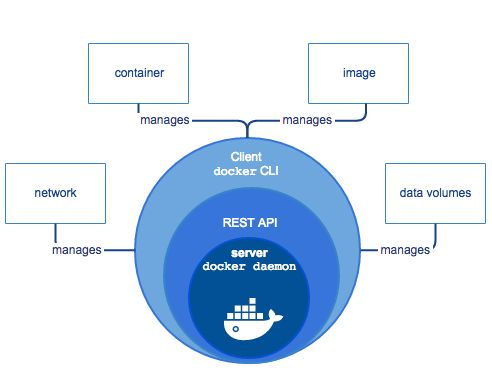
\includegraphics[width=\columnwidth]{./Figure/docker-048-041}
\end{center}
\end{frame}

\begin{frame}
\frametitle{Image --- Container}

\begin{itemize}
\item \textit{Image} is static, immutable
\item \textit{Container} is dynamic, mutable
\end{itemize}
\end{frame}

\begin{frame}
\frametitle{Image --- Container}

\begin{center}
1 container = 1 image\\
\vspace{0.5cm}
1 image = several containers
\end{center}
\end{frame}

 \frame{
  \frametitle {}
  \vspace{2cm}
  \centerline{\Huge \color{NavyBlue} \textbf{\emph{Command Line Interface}}}
}


\begin{frame}[fragile]
\frametitle{Simple commands}

To start a new container

\begin{lstlisting}
$ docker run -d -t ubuntu:18.04
\end{lstlisting}

\end{frame}

\begin{frame}[fragile]
\frametitle{Simple commands}

finds the container ID
\begin{lstlisting}
$ docker ps
\end{lstlisting}
lists the containers; the new container is on top of the list; grab the \textit{NAME}
\end{frame}

\begin{frame}[fragile]
\frametitle{Simple commands}

\begin{lstlisting}
$ docker exec suspicious_davinci "ls" "-lpF"
\end{lstlisting}
runs a command in the container, assuming the name is \textit{suspicious\_davinci}
\end{frame}

\begin{frame}[fragile]
\frametitle{RUN}
\scriptsize
\begin{lstlisting}[breaklines=true]
$ docker run --help

Usage:  docker run [OPTIONS] IMAGE [COMMAND] [ARG...]

Run a command in a new container

Options:
      --add-host list                  Add a custom host-to-IP mapping (host:ip)
  -a, --attach list                    Attach to STDIN, STDOUT or STDERR
      --blkio-weight uint16            Block IO (relative weight), between 10 and 1000, or 0 to disable (default 0)
      --blkio-weight-device list       Block IO weight (relative device weight) (default [])
      --cap-add list                   Add Linux capabilities
      --cap-drop list                  Drop Linux capabilities
      --cgroup-parent string           Optional parent cgroup for the container
      --cidfile string                 Write the container ID to the file
      --cpu-period int                 Limit CPU CFS (Completely Fair Scheduler) period
      --cpu-quota int                  Limit CPU CFS (Completely Fair Scheduler) quota
      --cpu-rt-period int              Limit CPU real-time period in microseconds

... very long list of options
\end{lstlisting}
\normalsize
\end{frame}

\begin{frame}[fragile]
\frametitle{RUN}
\framesubtitle{Detach}
\begin{lstlisting}
$ docker run -d -t ubuntu:18.04
\end{lstlisting}

\begin{itemize}
\item \lstinline!-d! option detached
\item \lstinline!-t! create a terminal
\item \lstinline!ubuntu! image
\item \lstinline!18.04! image version (label)
\end{itemize}
\end{frame}

\begin{frame}[fragile]
\frametitle{RUN}
\framesubtitle{Interactive}
\begin{lstlisting}
$ docker run -i -t ubuntu:18.04 /bin/bash
\end{lstlisting}

\begin{itemize}
\item \lstinline!-i! option interactive
\item \lstinline!-t! attached to your terminal
\item \lstinline!ubuntu! image
\item \lstinline!18.04! image version (label)
\item \lstinline!/bin/bash! program to run inside the container
\end{itemize}
When the program completes the execution, the container is stopped (but not deleted)
\end{frame}

\begin{frame}[fragile]
\frametitle{RUN}
\framesubtitle{remove container}
\begin{lstlisting}
$ docker run --rm hello-world
\end{lstlisting}
\lstinline!--rm! deletes the container (not the image)
\end{frame} 
 
\begin{frame}[fragile]
\frametitle{RUN}
\framesubtitle{naming a container}
\begin{lstlisting}
$ docker run -it --name vm ubuntu:18.04 /bin/bash
\end{lstlisting}

\begin{itemize}
\item \lstinline!-it! is like \lstinline!-i -t!
\item \lstinline!--name! use \textit{vm} for naming the new \textit{container}
\end{itemize}
Sometimes a random name is not a good idea\\
Names must be unique.
\end{frame}

\begin{frame}[fragile]
\frametitle{RUN}
\framesubtitle{host pid}
\begin{lstlisting}
$ docker run -it --rm --pid=host  ubuntu:18.04 top
\end{lstlisting}
\lstinline!--pid=host! the container and the host computer share the same process IDs (just like a native process)
\begin{columns}
\begin{column}{.50\textwidth}
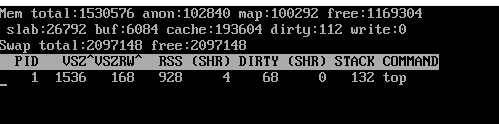
\includegraphics[width=\columnwidth]{./Figure/commands/pid-normal}
\end{column}
\begin{column}{.50\textwidth}
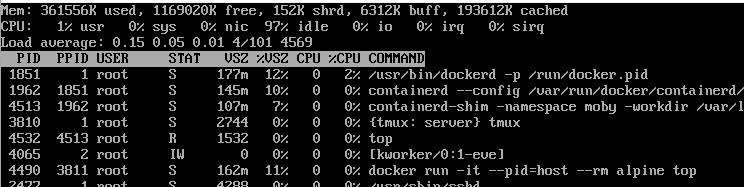
\includegraphics[width=\columnwidth]{./Figure/commands/pid-host}
\end{column}
\end{columns}
\end{frame}

\begin{frame}[fragile]
\frametitle{RUN}
\framesubtitle{limiting resources}
\begin{lstlisting}
$ docker run -dt --name vm -m 1g ubuntu:18.04 /bin/bash
\end{lstlisting}
\begin{itemize}
\item \lstinline!-m! max amount of memory available
\item \lstinline!--memory-swap! max amount of swap memory. If not specified is equal to the max memmory (in this case 1GB)
\item \lstinline!--cpus! number of cpus available. Can be a fraction
\end{itemize}
\end{frame}

\begin{frame}[fragile]
\frametitle{RUN}
\framesubtitle{command arguments}
\begin{lstlisting}
$ docker run -t  -m 1g ubuntu:18.04 ls -lph /var
\end{lstlisting}
Just place them after the command.
\end{frame}

\begin{frame}[fragile]
\frametitle{RUN}
\framesubtitle{environment}
\begin{lstlisting}
$ docker run -it -e "DEBUG=true" ubuntu:18.04 ls -lph /
\end{lstlisting}
Set the value of an environment variable.\\
\vspace{0.4cm}
A separate \lstinline!-e! for each variable.
\end{frame}

\begin{frame}[fragile]
\frametitle{RUN}
\framesubtitle{Detach from a running container}
\begin{lstlisting}
$ docker run --rm -it --name Duck ubuntu:18.04 /bin/bash
\end{lstlisting}
Detach from the container using \lstinline!Ctrl-P! + \lstinline!Ctrl-Q!
\end{frame}

\begin{frame}[fragile]
\frametitle{RUN}
\framesubtitle{ReAttach to a running container}
\begin{lstlisting}
$ docker attach Duck
\end{lstlisting}
\end{frame}

\begin{frame}[fragile]
\frametitle{Processes}
\scriptsize
\begin{lstlisting}[breaklines=true]
$ docker ps --help

Usage:  docker ps [OPTIONS]

List containers

Options:
  -a, --all             Show all containers (default shows just running)
  -f, --filter filter   Filter output based on conditions provided
      --format string   Pretty-print containers using a Go template
  -n, --last int        Show n last created containers (includes all states) (default -1)
  -l, --latest          Show the latest created container (includes all states)
      --no-trunc        Don't truncate output
  -q, --quiet           Only display numeric IDs
  -s, --size            Display total file sizes
\end{lstlisting}
\normalsize
\end{frame}

\begin{frame}[fragile]
\frametitle{Processes}
\begin{lstlisting}
$ docker ps
\end{lstlisting}
List the running containers 
\begin{lstlisting}
$ docker ps -a
\end{lstlisting}
List all containers 
\end{frame}


\begin{frame}[fragile]
\frametitle{RUN}
\framesubtitle{ReAttach to a running container}
Using the container \textit{id}
\end{frame}


\begin{frame}[fragile]
\frametitle{EXEC}
\scriptsize
\begin{lstlisting}[breaklines=true]
$ docker exec --help

Usage:  docker exec [OPTIONS] CONTAINER COMMAND [ARG...]

Run a command in a running container

Options:
  -d, --detach               Detached mode: run command in the background
      --detach-keys string   Override the key sequence for detaching a container
  -e, --env list             Set environment variables
  -i, --interactive          Keep STDIN open even if not attached
      --privileged           Give extended privileges to the command
  -t, --tty                  Allocate a pseudo-TTY
  -u, --user string          Username or UID (format: <name|uid>[:<group|gid>])
  -w, --workdir string       Working directory inside the container
\end{lstlisting}
\normalsize
\end{frame}

\begin{frame}[fragile]
\frametitle{EXEC}
\begin{lstlisting}
$ docker exec vm df -h
\end{lstlisting}

Runs a command (in this case \lstinline!df -h!) in a running container
\end{frame}

\begin{frame}[fragile]
\frametitle{IMAGES}
\scriptsize
\begin{lstlisting}[breaklines=true]
$ docker images --help

Usage:  docker images [OPTIONS] [REPOSITORY[:TAG]]

List images

Options:
  -a, --all             Show all images (default hides intermediate images)
      --digests         Show digests
  -f, --filter filter   Filter output based on conditions provided
      --format string   Pretty-print images using a Go template
      --no-trunc        Don't truncate output
  -q, --quiet           Only show numeric IDs
\end{lstlisting}
\normalsize
\end{frame}


\begin{frame}[fragile]
\frametitle{IMAGES}
\begin{lstlisting}
$ docker images
\end{lstlisting}

List the images 
\end{frame}

\begin{frame}[fragile]
\frametitle{IMAGE}
\scriptsize
\begin{lstlisting}[breaklines=true]
$ docker image --help

Usage:  docker image COMMAND
Manage images

Options:

Commands:
  build       Build an image from a Dockerfile
  history     Show the history of an image
  import      Import the contents from a tarball to create a filesystem image
  inspect     Display detailed information on one or more images
  load        Load an image from a tar archive or STDIN
  ls          List images
  prune       Remove unused images
  pull        Pull an image or a repository from a registry
  push        Push an image or a repository to a registry
  rm          Remove one or more images
  save        Save one or more images to a tar archive (streamed to STDOUT by default)
  tag         Create a tag TARGET_IMAGE that refers to SOURCE_IMAGE

Run 'docker image COMMAND --help' for more information on a command.
\end{lstlisting}
\normalsize
\end{frame}

\begin{frame}[fragile]
\frametitle{IMAGE}
\framesubtitle{inspect}
\begin{lstlisting}
$ docker image inspect hello-world
\end{lstlisting}

Gives several information on the image
\end{frame}


\begin{frame}[fragile]
\frametitle{Remove Image}
\begin{lstlisting}
$ docker rmi hello-world
\end{lstlisting}

Deletes a local image. It has no effect on the hub.
\end{frame}

\begin{frame}[fragile]
\frametitle{Remove container}
\scriptsize
\begin{lstlisting}[breaklines=true]
$ docker rm --help

Usage:  docker rm [OPTIONS] CONTAINER [CONTAINER...]

Remove one or more containers

Options:
  -f, --force     Force the removal of a running container (uses SIGKILL)
  -l, --link      Remove the specified link
  -v, --volumes   Remove the volumes associated with the container
\end{lstlisting}
\normalsize
\end{frame}

\begin{frame}[fragile]
\frametitle{Remove container}
\begin{lstlisting}
$ docker rm vm
\end{lstlisting}
Deletes a container and all its data (volumes) 
\end{frame}

\begin{frame}[fragile]
\frametitle{System pruning}
\begin{lstlisting}
$ docker system prune
\end{lstlisting}

Reclaim all disk space
\end{frame}

\begin{frame}[fragile]
\frametitle{System}
\scriptsize
\begin{lstlisting}[breaklines=true]
$ docker system --help

Usage:  docker system COMMAND
Manage Docker
Options:

Commands:
  df          Show docker disk usage
  events      Get real time events from the server
  info        Display system-wide information
  prune       Remove unused data

Run 'docker system COMMAND --help' for more information on a command.
\end{lstlisting}
\normalsize
\end{frame}

\begin{frame}[fragile]
\frametitle{Disk space}
\begin{lstlisting}
$ docker system df
\end{lstlisting}
Shows what is using disk space
\end{frame}

\begin{frame}[fragile]
\frametitle{PULL}
\scriptsize
\begin{lstlisting}[breaklines=true]
$ docker pull --help

Usage:  docker pull [OPTIONS] NAME[:TAG|@DIGEST]

Pull an image or a repository from a registry

Options:
  -a, --all-tags                Download all tagged images in the repository
      --disable-content-trust   Skip image verification (default true)
\end{lstlisting}
\normalsize
\end{frame}

\begin{frame}[fragile]
\frametitle{PULL}
\begin{lstlisting}
$ docker pull ubuntu:14.08
\end{lstlisting}

Download from the public repository a desired image
\end{frame}

\begin{frame}[fragile]
\frametitle{COMMIT}
Transforming a container into an image.
\begin{itemize}
\item run a container w/o \lstinline!--rm!
\item install some software
\item exit from the container
\item remember the container id
\item commit the change.
\end{itemize}
\end{frame}

\begin{frame}[fragile]
\frametitle{COMMIT}
\framesubtitle{Transform a container into an image.}
\scriptsize
\begin{lstlisting}[breaklines=true]
$ docker commit --help
Usage:  docker commit [OPTIONS] CONTAINER [REPOSITORY[:TAG]]

Create a new image from a container s changes

Options:
  -a, --author string      Author (e.g., John Hannibal Smith <hannibal@a-team.com>)
  -c, --change list         Apply Dockerfile instruction to the created image
  -m, --message string Commit message
  -p, --pause                Pause container during commit (default true)
\end{lstlisting}
\normalsize
\end{frame}

\begin{frame}[fragile]
\frametitle{COMMIT}
\framesubtitle{Transform a container into an image.}
\scriptsize
\begin{lstlisting}[breaklines=true]
$ docker run -it ubuntu:18.04 sh -c apt update && apt install git

$ docker ps -a
CONTAINER ID  IMAGE           COMMAND                  NAMES
8bb0b797af88   ubuntu:18.04 sh -c ''apt update''       condescending_shaw

$ docker commit -m install git 8bb0b797af88 ubuntu_git:0.1
sha256:c47472e998a05687938fc9a5ebfa6cfbfff137aeb360b37de00e99515ab0298a

$ docker images | head
REPOSITORY  TAG IMAGE ID         SIZE
ubuntu_git      0.1  c47472e998a0 212MB
\end{lstlisting}
\normalsize
\end{frame}


%    \frame{
%\frametitle{Docker hub} 
% 
%     	\begin{center}
%  			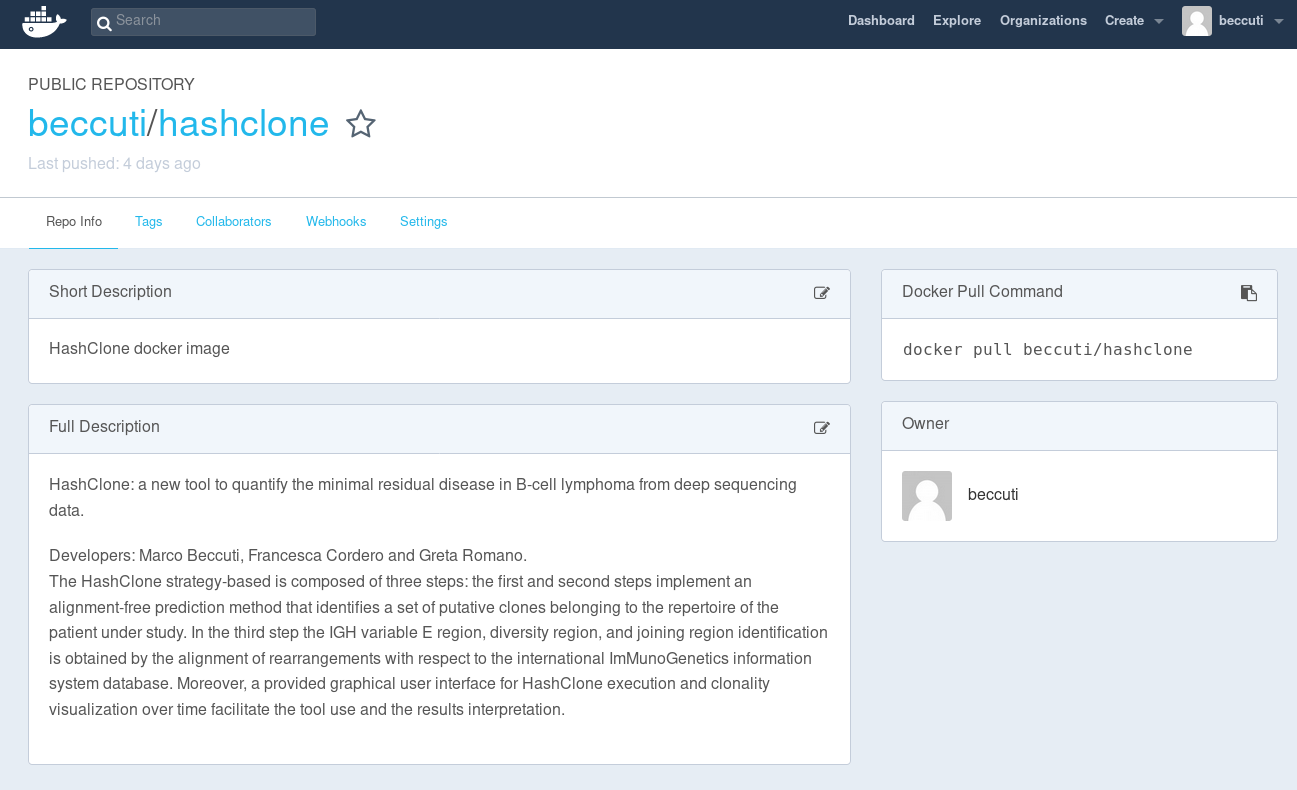
\includegraphics[width=1.00\columnwidth]{./Figure/hub}
%  		\end{center}  
%  
% }
  
  
  
  

 \frame{
  \frametitle {}
  \vspace{2cm}
  \centerline{\Huge \color{NavyBlue} \textbf{\emph{Our first simple Docker image}}}
  
     	\begin{center}
  			
\includegraphics[width=0.50\columnwidth]{./Figure/dockersimple}
  		\end{center} 
}
 
  
  \frame{
  \frametitle {Our first simple Docker image}
 To create our image we will perform the following tasks:\vspace{0.4cm}
 \begin{itemize}
 \item Create an own docker public repository;\vspace{0.2cm}	
 \item Download a  base image from the Docker Hub;\vspace{0.2cm}	
 \item Updating the download image and upload it on our own repository;\vspace{0.2cm}	
 \item Create and embed  simple BASH and R  scripts on our image;\vspace{0.2cm}	
 \item Execute the new created image.
 \end{itemize}
}
  
    \frame{
  \frametitle {Our first simple Docker image}
 To create our image we will perform the following tasks:\vspace{0.4cm}
 \begin{itemize}
 \item Create an own docker public repository;\vspace{0.2cm}\color{grey}	
 \item Download a  base image from the Docker Hub;\vspace{0.2cm}	
 \item Updating the download image and upload it on our own repository;\vspace{0.2cm}	
 \item Create and embed  simple BASH and R  scripts on our image;\vspace{0.2cm}	
 \item Execute the new created image.
 \end{itemize}
} 
 
  
   \frame{
  \frametitle { Create an own docker public repository}
  We have to create a free \textbf{\color{NavyBlue}docker ID} at the following address: \color{NavyBlue}\url{ https://hub.docker.com/}
  
       	\begin{center}
  			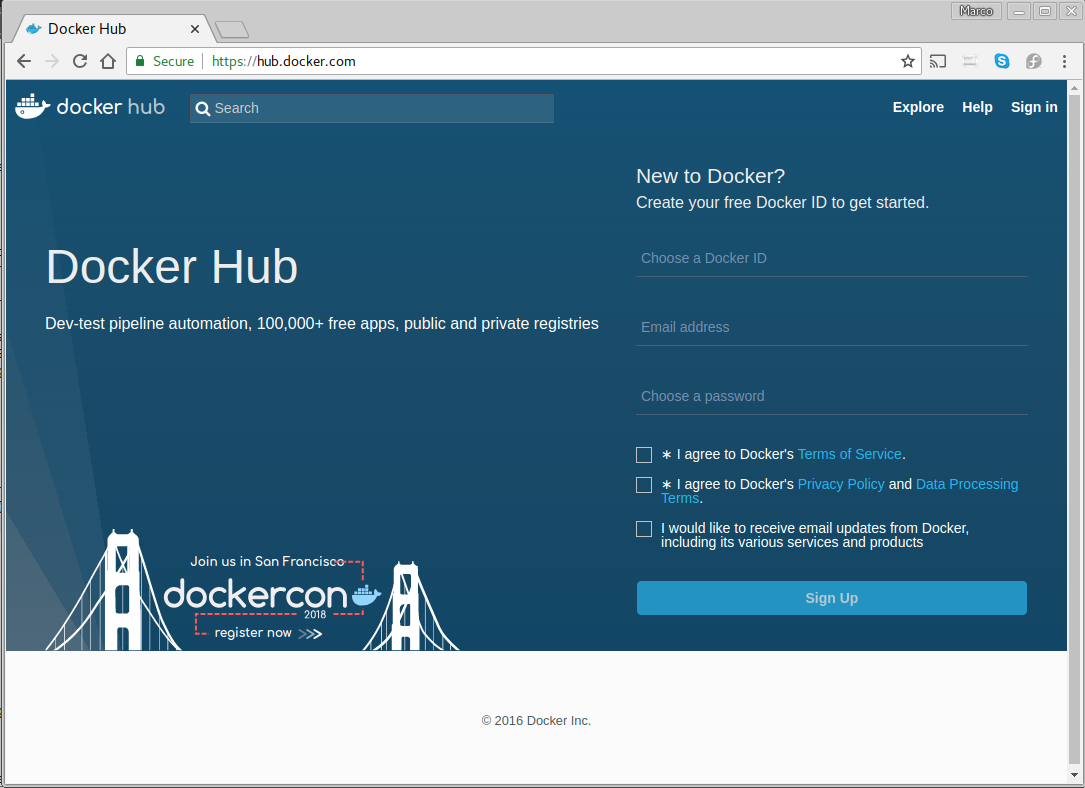
\includegraphics[width=0.60\columnwidth]{./Figure/dockerhub}
  		\end{center}  
  
  
  
  }
    
   \frame{
  \frametitle { Create an own docker public repository}
  We have to create a  \textbf{\color{NavyBlue}public repository} 
  
       	\begin{center}
  			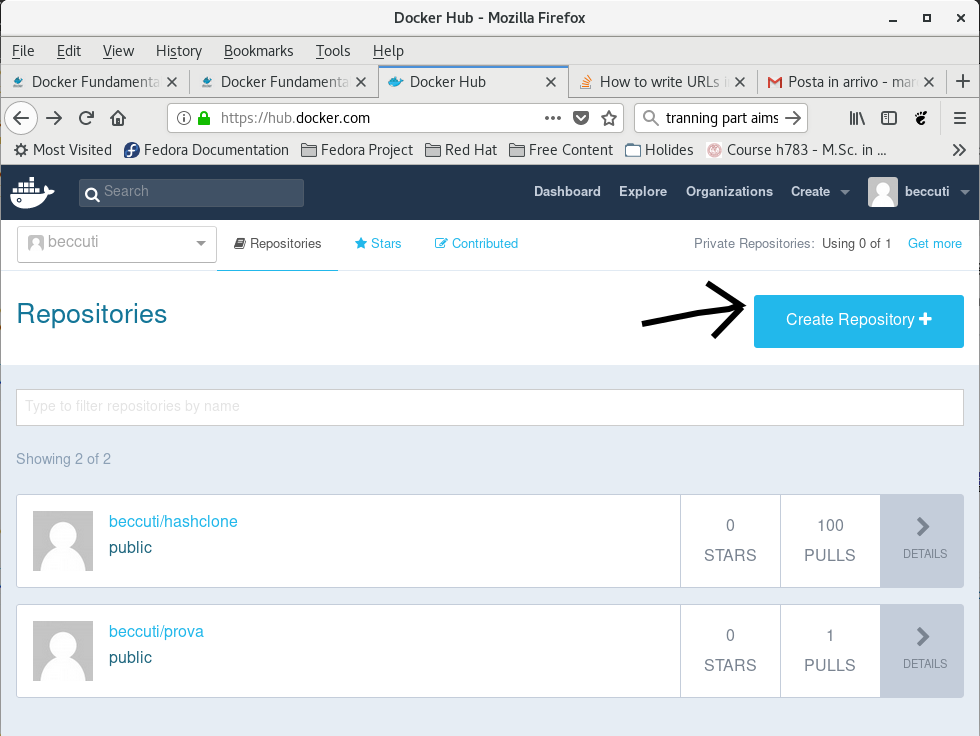
\includegraphics[width=0.60\columnwidth]{./Figure/dockerhub1}
  		\end{center}  
  }
  
    
     \frame{
  \frametitle { Create an own docker public repository}\vspace{0.2cm}
  We have to create a  \textbf{\color{NavyBlue}public repository} 
  
       	\begin{center}
  			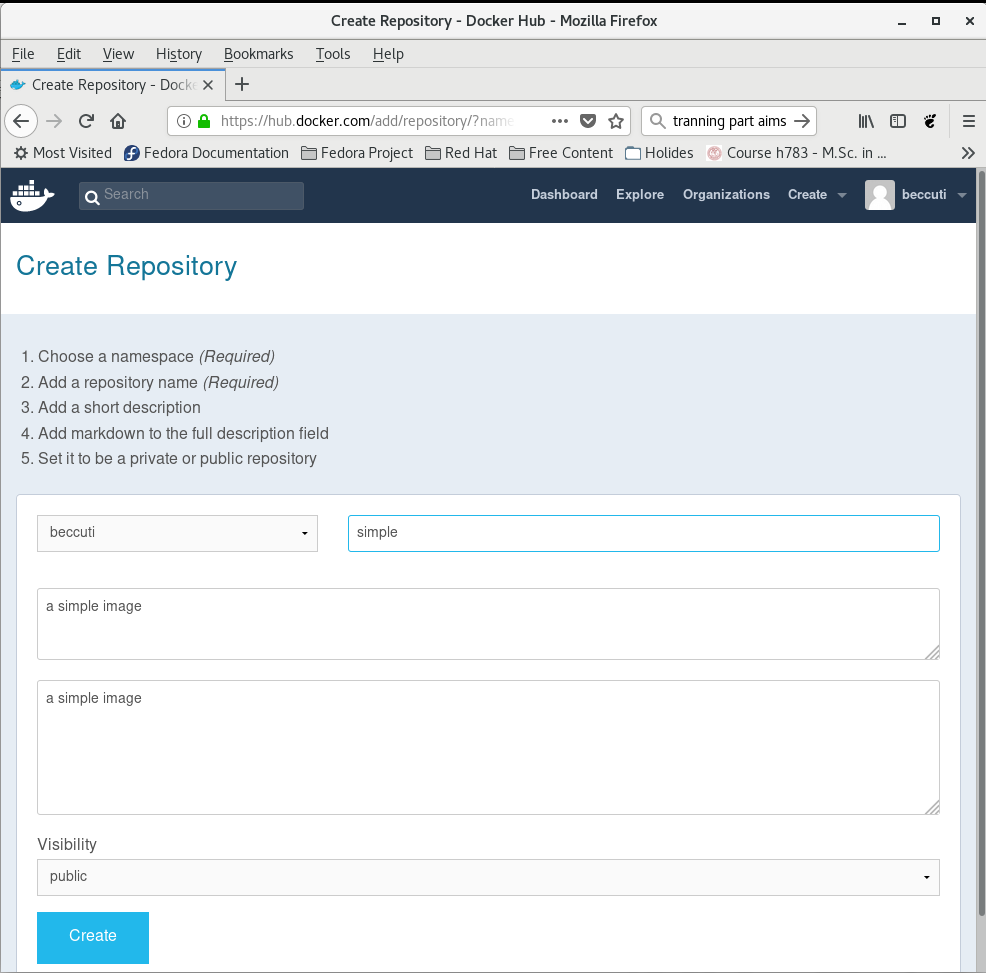
\includegraphics[width=0.63\columnwidth]{./Figure/dockerhub2}
  		\end{center}  
  
  
  
  }
  
       \frame{
  \frametitle { Create an own docker public repository}
  \begin{itemize}
  \item Collaborators can be added;\vspace{0.2cm}
  \item Image id is: \emph{\color{NavyBlue}$\langle$docker\_ID$\rangle$/$\langle$image\_ID$\rangle$} 
  \end{itemize}
       	\begin{center}
  			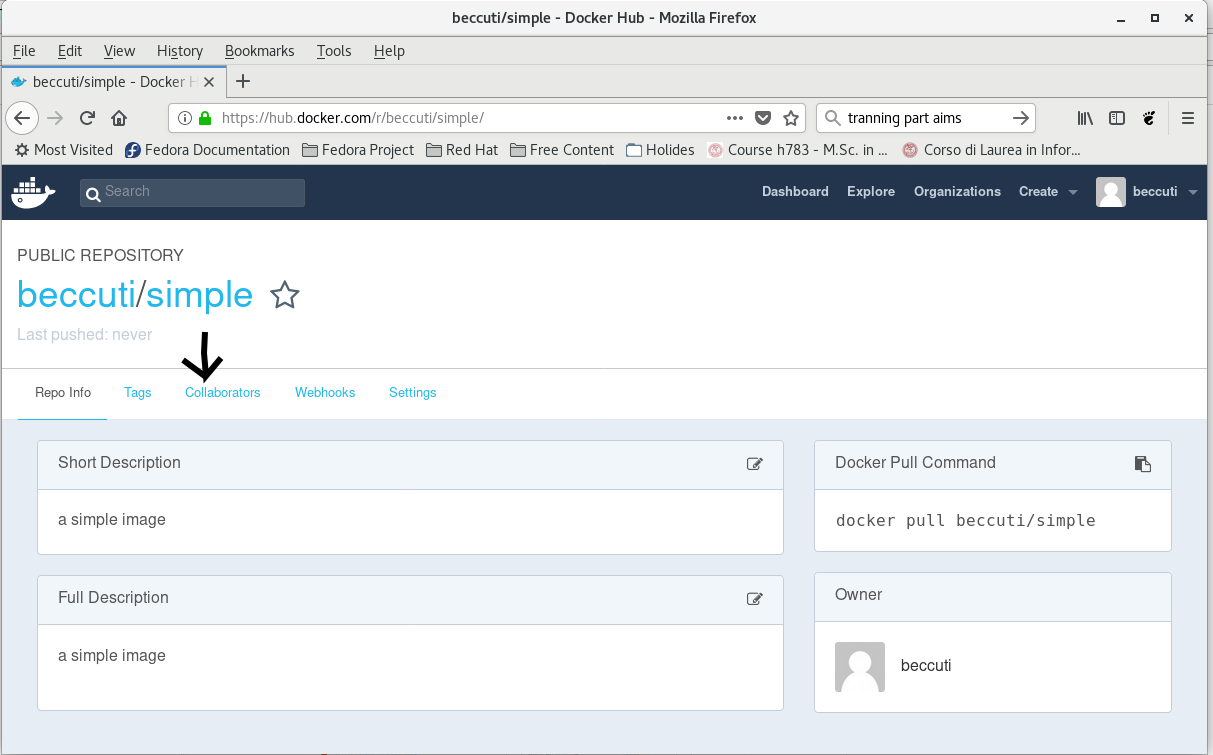
\includegraphics[width=0.85\columnwidth]{./Figure/dockerhub3}
  		\end{center}  
  }
  
 
  \frame{
  \frametitle {Our first simple Docker image}
 To create our image we will perform the following tasks:\vspace{0.4cm}
 \begin{itemize}
 \item Create an own docker public repository;\vspace{0.2cm}
 \item Download a  base image from the Docker Hub;\vspace{0.2cm}	\color{grey}	
 \item Updating the download images and upload it on our own repository;\vspace{0.2cm}	
 \item Create and embed  simple BASH and R  scripts on our image;\vspace{0.2cm}	
 \item Execute the new created image.
 \end{itemize}
} 


   \frame{
  \frametitle {Download a  base image from the Docker Hub}
  We can access the docker documentation at following address: \color{NavyBlue}\url{https://docs.docker.com/}
  
       	\begin{center}
  			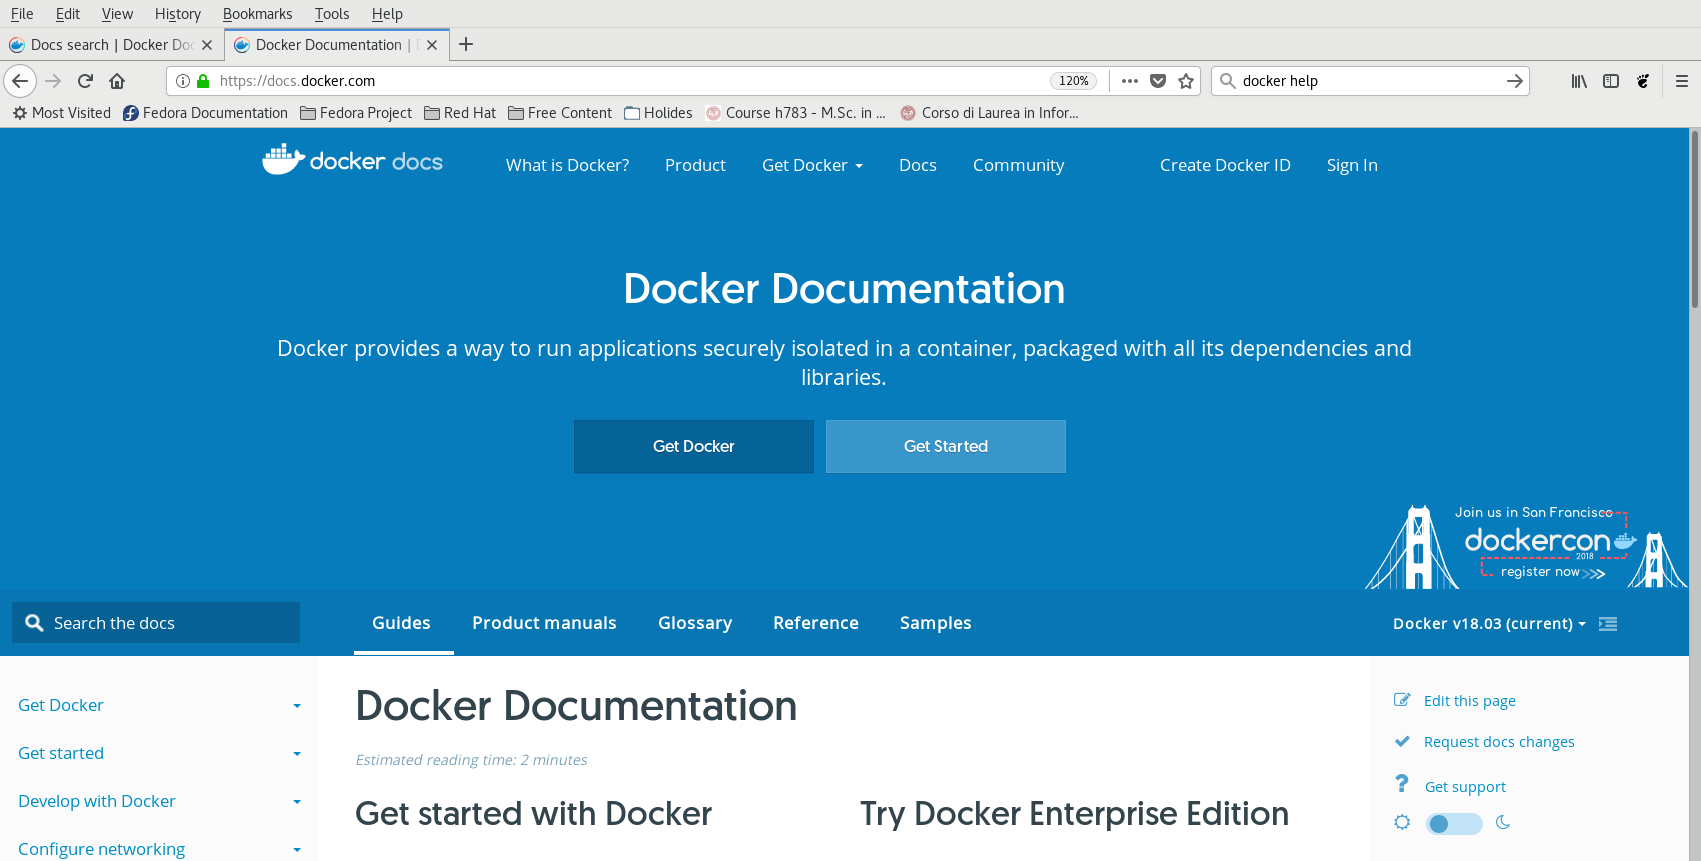
\includegraphics[width=1.00\columnwidth]{./Figure/dockerDoc}
  		\end{center}  
  
  
  
  }
 
  \frame{
  \frametitle {Download a  base image from the Docker Hub}  
 \emph{\color{PineGreen} docker pull 
 $\langle \it{image} \rangle$} can be used to download a docker image from  a hub.
     	\begin{center}
  			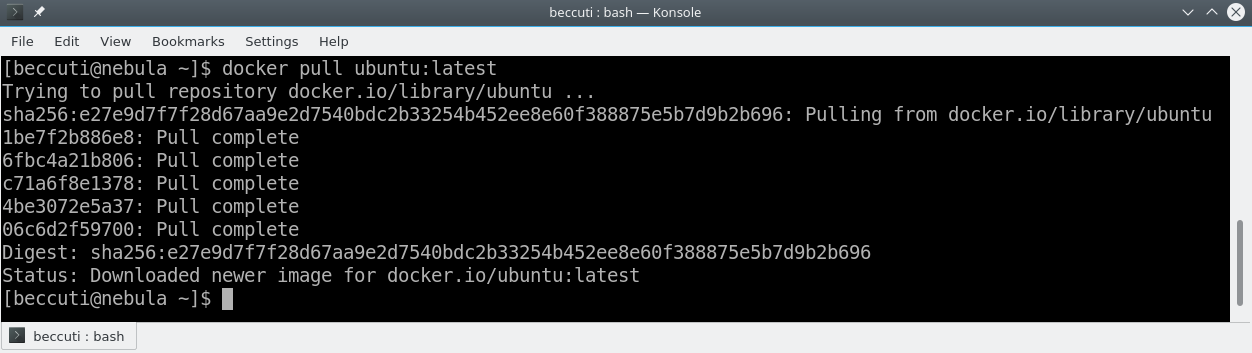
\includegraphics[width=1.00\columnwidth]{./Figure/pull}
  		\end{center}  
 \begin{itemize}
 \item  tags (i.e. \emph{\color{NavyBlue}:$\langle$tag\_name$\rangle$}) can be exploited to choice among different image releases;\vspace{0.2cm}
 \item different releases can \textbf{\color{NavyBlue}share layers} (common image portions) to save disk space;\vspace{0.2cm}
 \item  If no tag is provided, Docker Engine uses the  \emph{\color{NavyBlue}:latest} tag as a default.
 \end{itemize} 
  
 }
 
 
     \frame{
\frametitle{Download a  base image from the Docker Hub} 
  
 \emph{\color{PineGreen} docker images} can be used to list the Docker images installed on a machine. 
     	\begin{center}
  			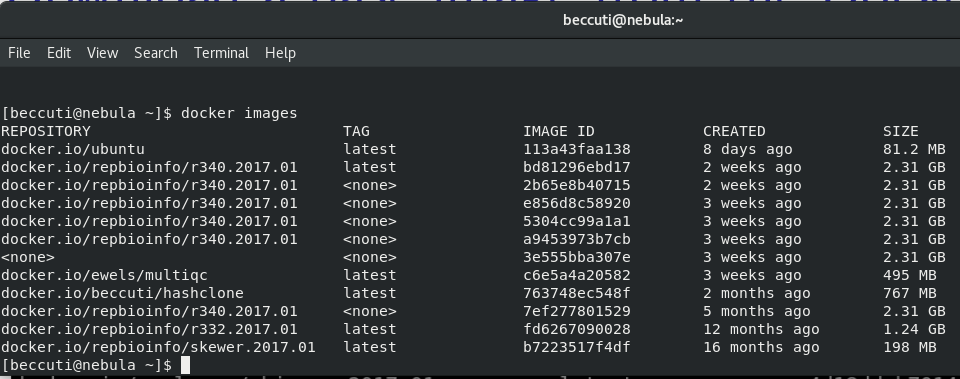
\includegraphics[width=1.00\columnwidth]{./Figure/dockerimages}
  		\end{center}  
  \begin{itemize}
  \item \emph{\color{NavyBlue} <none>:<none>} images are the dangling images which may cause disk space problems;
  \vspace{0.2cm}
  \item Docker does not have an automatic garbage collection system as of now;
   
  \end{itemize}
 }
 
       \frame{
\frametitle{Download a  base image from the Docker Hub} 
  
 \emph{\color{PineGreen} docker rmi 
 $\langle \it{image} \rangle$} can be used to remove a docker image.
     	\begin{center}
  			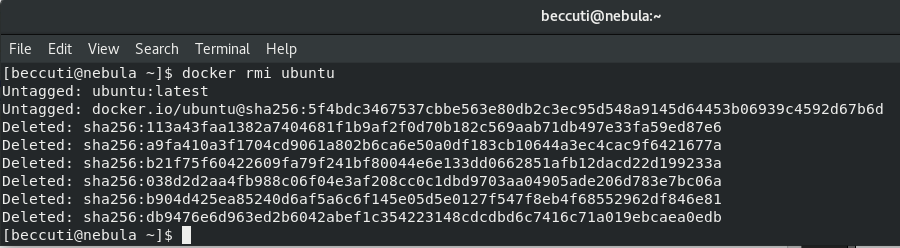
\includegraphics[width=0.97\columnwidth]{./Figure/rm}
  		\end{center}  
  
All \emph{\color{NavyBlue}dangling images} can be removed combining the following two docker commands: 	
 
      	\begin{center}
  			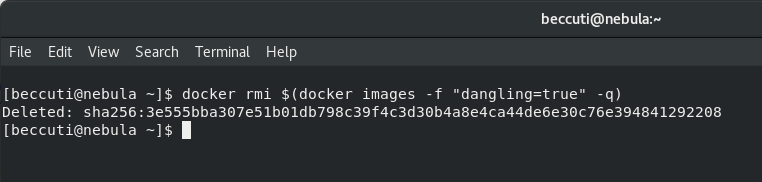
\includegraphics[width=0.97\columnwidth]{./Figure/rm1}
  		\end{center} \vspace{-0.1cm}
 where option \emph{\color{PineGreen}-f "dangling=true"} filters  all the dangling images  and \emph{\color{PineGreen} -q}   returns only docker id.		
 } 	 	
 
       \frame{
\frametitle{Download a  base image from the Docker Hub}  
 	If an image has one or more dependencies, you must remove all of them before.
       	\begin{center}
  			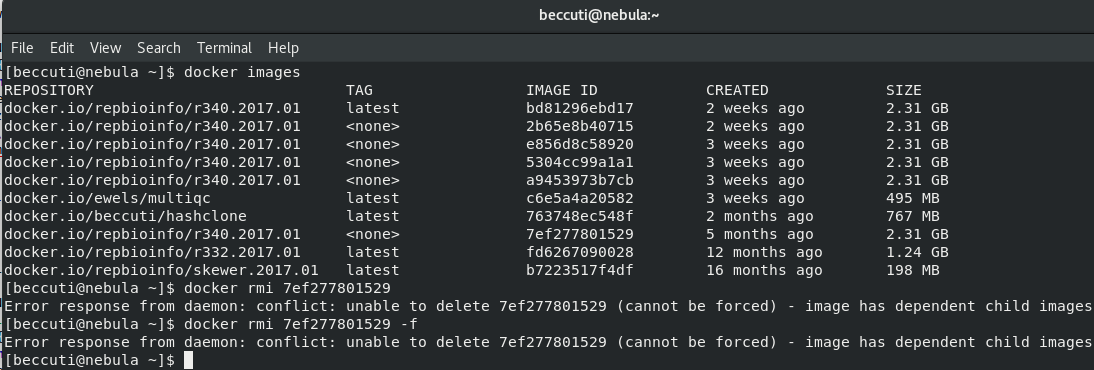
\includegraphics[width=1.02\columnwidth]{./Figure/rm2}
  		\end{center}
}  		

       \frame{
\frametitle{Download a  base image from the Docker Hub}    		
 \emph{\color{PineGreen} docker image history} can be used to list the history of Docker image.  		
        	\begin{center}
  			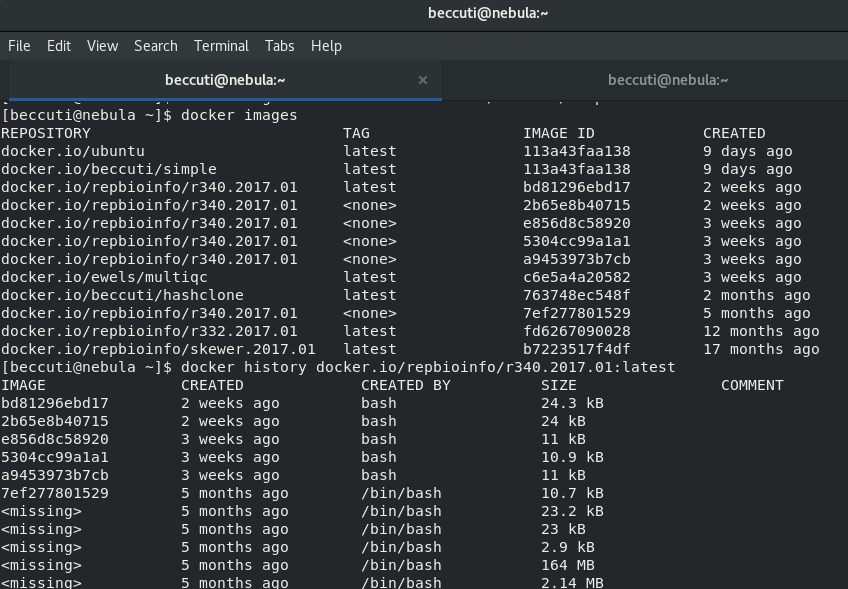
\includegraphics[width=0.90\columnwidth]{./Figure/history}
  		\end{center}%\vspace{-0.2cm}
 Observe that  \textbf{\color{NavyBlue} missing} is for no local dependencies. 		
}  		
  

\frame{
\frametitle {}
\vspace{2cm}
\centerline{\Huge \color{NavyBlue} \textbf{\emph{Volumes}}}
\vspace{0.5cm}
}
\frame{
\frametitle{Data in Docker}
We are in a containerized world.\\
Everything is separated.\\
How do we share/access data ?\\
}

\frame{
\frametitle{Data in Docker: Goals}
\begin{itemize}
\item How Docker manages data ?
\item Use different type of data storage
\end{itemize}
}

\frame{
\frametitle{Data in Docker}
Docker has 3 options
\begin{itemize}
\item Volumes
\item Bind Mounts
\item tmpfs mount
\end{itemize}
}


\frame{
\frametitle{Data in Docker}
Docker and data
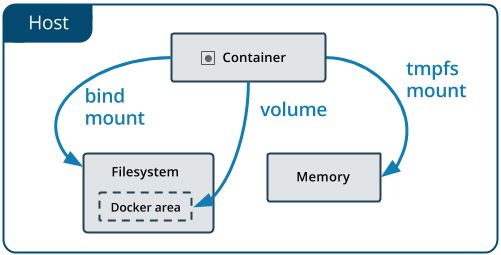
\includegraphics[width=0.50\columnwidth]{./Figure/docker-080-054}
}

\frame{
\frametitle{Data in Docker}
\framesubtitle{Volumes}
\begin{itemize}
\item Managed directly by Docker
\item Saved in \lstinline!/var/lib/docker/volumes/! on the host
\item System processes can not access data outside Docker
\item Recommended by Docker to store data in Docker
\end{itemize}
}

\frame{
\frametitle{Data in Docker}
\framesubtitle{Volumes}

\begin{itemize}
\item User can create its own volumes or instruct Docker to create them when required by the containers or services
\item The container see the volume as a directory and the user define the name
\item Docker guarantees isolation from the host machine
\item A volume can be mounted by many containers at the same time
\end{itemize}
}

\frame{
\frametitle{Data in Docker}
\framesubtitle{Volumes}
\begin{itemize}
\item If not used it is not destroyed, the user must remove the volume explicitly
\item The user can name a volume or Docker create a random name automatically
\item A volume can be an \it{object} in the cloud, the user must use a proper \it{driver}
\item Avoid to increase the size of the container
\end{itemize}
}

\frame{
\frametitle{Data in Docker}
\framesubtitle{Bind mounts}

\begin{itemize}
\item Managed directly by the host OS
\item Saved in  \emph{\color{PineGreen} /in/your/path/} on the host OS
\item System processes or Docker containers can access to the data
\item It is possible to override important files or directory on the host OS
\end{itemize}

}

\frame{
\frametitle{Data in Docker}
\framesubtitle{Bind mounts}

\begin{itemize}
\item Files and directory from the host are mounted inside the container at runtime
\item Require the target's full path on the host machine
\item On demand creation inside the container
\item Very performant
\item Rely on the host filesystem
\item From inside the contianer the user has full access to the filesystem: read/write
\item Read/Write from outside the Docker container
\end{itemize}
}

\frame{
\frametitle{Data in Docker}

Expose a \it{Volume} or \it{Bind Mount} into the container

 \emph{\color{PineGreen} --volume | -v}

Docker infers if it is a \it{Volume} or a \it{Bind Mount} from the command line
}

\frame{
\frametitle{Data in Docker}

In memory storage

 \emph{\color{PineGreen} --tmpfs}

This is useful for ephemeral storage
}

\begin{frame}[fragile]
\frametitle{Data in Docker}
\framesubtitle{When use What}

\begin{itemize}
\item \textit{Volume}
  \begin{itemize}
  \item Sharing data among containers
  \item The host lacks a directory structure
  \item Data can not be stored locally (cloud)
  \end{itemize}
\item \textit{Bind mount}
  \begin{itemize}
  \item Sharing configuration to containers
  \item Sharing source code and build products
  \item Stable directory and file structures shared w/ containers
  \end{itemize}
\end{itemize}
\end{frame}

\begin{frame}[fragile]
\frametitle{Data in Docker}
\framesubtitle{CLI}

\begin{lstlisting}
 docker volume

Commands:
  create   Create a volume
  inspect  Display detailed information on one or more
           volumes
  ls       List volumes
  prune    Remove all unused volumes
  rm       Remove one or more volumes
\end{lstlisting}
\end{frame}


\begin{frame}[fragile]
\frametitle{Data in Docker}
\framesubtitle{Create a volume}

\begin{lstlisting}
$ docker volume create edr19-storage

edr19-storage
\end{lstlisting}
\end{frame}

\begin{frame}[fragile]
\frametitle{Data in Docker}
\framesubtitle{List volumes}


\begin{lstlisting}
$ docker volume ls

DRIVER    VOLUME NAME
local     edr19-storage
\end{lstlisting}
\end{frame}

\begin{frame}[fragile]
\frametitle{Data in Docker}
\framesubtitle{Inspecting a volume}
\begin{lstlisting}[breaklines=true]
$ docker volume inspect edr19-storage

[{
  "CreatedAt": "2019-05-20T18:38+00:00",
  "Driver": "local",
  "Labels": {},
  "Mountpoint": "/var/lib/docker/volumes/edr19-storage/_data",
  "Name": "edr19-storage",
  "Options": {},
  "Scope": "local"
  }]
\end{lstlisting}

\end{frame}

\begin{frame}[fragile]
\frametitle{Data in Docker}
\framesubtitle{Use a volume}

Run a container with Ubuntu 18.04 and create a file with something inside
\begin{lstlisting}
$ docker run --rm \
             -v edr19-storage:/data \
             -it ubuntu:18.04 /bin/bash 
$ echo $RANDOM > /data/seed
$ exit
\end{lstlisting}

After closing the container data are stored an can be accessed
by another container

\begin{lstlisting}
$ docker run --rm \
             -v edr19-storage:/data \
             -it ubuntu:18.04 /bin/bash \
             -c "cat /data/seed"
\end{lstlisting}
\end{frame}

\begin{frame}[fragile]
\frametitle{Data in Docker}
\framesubtitle{Mount points}

Load your own directory inside the container

\begin{lstlisting}
$ docker run -v /opt:/host/opt \
             --name edr19 \
             --rm \
             -it ubuntu:18.04 /bin/bash
\end{lstlisting}
\end{frame}

\begin{frame}[fragile]
\frametitle{Data in Docker}
\framesubtitle{Mount points}

Load your own directory inside the container

\begin{lstlisting}
$ docker run -v /opt:/host/opt \
             --name edr19 \
	      --rm \
            -it ubuntu:18.04 /bin/bash

\end{lstlisting}

\it{Docker does not like relative path}
\end{frame}

\begin{frame}[fragile]
\frametitle{Data in Docker}
\framesubtitle{Volumes and Mount points}

Combine volumes and mount points in a single instance

\begin{lstlisting}
$ docker run -v /opt:/host/opt \
             -v edr19-storage:/data \
             --name edr19 \
             --rm \
             -it ubuntu:18.04 /bin/bash
\end{lstlisting}
\end{frame}

\begin{frame}[fragile]
\frametitle{Data in Docker}
\framesubtitle{Share data w/ containers}


\begin{lstlisting}
$ docker run -v /opt:/host/opt \
             -v edr19-storage:/data \
             --name edr19 \
             --rm \
             -it ubuntu:18.04 /bin/bash

\end{lstlisting}
Another container can access to the data at the same time
\begin{lstlisting}
$ docker run --volumes-from edr19 \
             --name backup \
             --rm \
             -it ubuntu:18.04 /bin/bash
\end{lstlisting}
\it{You may notice some lag in updating data, it depends on the underlying Docker filesystem}
\end{frame}

\begin{frame}[fragile]
\frametitle{Data in Docker}
\framesubtitle{Share data w/ containers}

\scriptsize
\begin{lstlisting}
$ docker run -v /opt:/host/opt \
             -v edr19-storage:/data \
             --name edr19 \
             --rm \
             -it ubuntu:18.04 /bin/bash
\end{lstlisting}
\normalsize
Another container can access to the data and perform a backup automatically
\scriptsize
\begin{lstlisting}
$ docker run --volumes-from edr19 \
             --name backup \
            --rm \
            -it ubuntu:18.04 \
            tar vcz /host/opt/backup.tar.gz /data
\end{lstlisting}
\normalsize
\it{You may notice some lag in updating data, it depends on the underlying Docker filesystem}
\end{frame}

\begin{frame}[fragile]
\frametitle{Data in Docker}
\framesubtitle{Volumes on the fly}

When needed you can even create a Volume at runtime w/o using the explicit \lstinline{create} command. 

\begin{lstlisting}
$ docker run -v bioinfo:/reads \
             -v /opt:/host/opt \
             -v edr19-storage:/data \
             --name edr19 \
             --rm \
             -it ubuntu:18.04 /bin/bash
\end{lstlisting}
\end{frame}

\begin{frame}[fragile]
\frametitle{Data in Docker}
\framesubtitle{Volumes on the fly}

When needed you can even create a Volume at runtime w/o using the explicit \lstinline{create} command. 

\begin{lstlisting}
$ docker volume ls

DRIVER    VOLUME NAME
local     edr19-storage
local     bioinfo
\end{lstlisting}
\end{frame}

\begin{frame}[fragile]
\frametitle{Data in Docker}
\framesubtitle{Anonymous Volumes} 

When needed you can even create a Volume at runtime w/o using the explicit \lstinline{create} command. 

\begin{lstlisting}
$ docker run -v /anonymous \
             -v bioinfo:/reads \
             -v /opt:/host/opt \
             -v edr19-storage:/data \
             --name edr19 \
             --rm \
             -it ubuntu:18.04 /bin/bash
\end{lstlisting}
\end{frame}

\begin{frame}[fragile]
\frametitle{Data in Docker}
\framesubtitle{Anonymous Volumes}

When needed you can even create a Volume at runtime w/o using the explicit \lstinline{create} command. 

\begin{lstlisting}
$ docker volume ls

DRIVER    VOLUME NAME
local     edr19-storage
local     bioinfo
\end{lstlisting}

\it{Once exited from the container, there is no evidence about the anonymous container}
\end{frame}

\begin{frame}[fragile]
\frametitle{Data in Docker}
\framesubtitle{Anonymous Volumes}

w/o \lstinline{--rm}

When needed you can even create a Volume at runtime w/o using the explicit \lstinline!create! command. 


\begin{lstlisting}
$ docker run -v /anonymous \
             -v bioinfo:/reads \
             -v /opt:/host/opt \
             -v edr19-storage:/data \
             --name edr19 \
             -it ubuntu:18.04 /bin/bash
\end{lstlisting}
\end{frame}

\begin{frame}[fragile]
\frametitle{Data in Docker}
\framesubtitle{Anonymous Volumes}
 w/o \lstinline{--rm}

When needed you can even create a Volume at runtime w/o using the explicit \lstinline{create} command. 


\begin{lstlisting}
$ docker volume ls

DRIVER    VOLUME NAME
local     edr19-storage
local     bioinfo
local     8a76g20jc0gcbgf3952gbdnihd253r801skala7898y...
\end{lstlisting}
\end{frame}

\begin{frame}[fragile]
\frametitle{Data in Docker}
\framesubtitle{Tech notes}

Docker \it{volumes}, \it{images}, \it{container} are capped to a defaul value which is configured at daemon level usually around \texttt{10 GB}

\begin{lstlisting}
dm.basesize
\end{lstlisting}
\end{frame}

\frame{
\frametitle{Data in Docker}
\framesubtitle{Tech notes}

The \lstinline{dm.basesize} can be increased but the Docker's daemon must be restared.
}

\begin{frame}[fragile]
\frametitle{Data in Docker}
\framesubtitle{Tech notes}

The user can run the daemon by hand 
\begin{lstlisting}
$ sudo dockerd --storage-opt dm.basesie=50G
\end{lstlisting}
\end{frame}

\frame{
\frametitle{Data in Docker}
\framesubtitle{Tech notes}

The user can increase the size but never decrease it.

If the user specifes a value which is lower than the minimum size of \it{volumes}, \it{images}, \it{containers} Docker will complain with errors.
}

\begin{frame}[fragile]
\frametitle{Data in Docker}
\framesubtitle{Tech notes}

Usually everything works fine, but may happend that Docker' system dir should be wiped out
\begin{lstlisting}
$ sudo service docker stop

$ sudo rm -rf /var/lib/docker
\end{lstlisting}
\end{frame}

 \frame{
  \frametitle {}
  \vspace{2cm}
  \centerline{\Huge \color{NavyBlue} \textbf{\emph{Our first simple Docker image}}}
  
     	\begin{center}
  			
\includegraphics[width=0.50\columnwidth]{./Figure/dockersimple}
  		\end{center} 
}


   \frame{
  \frametitle {Our first simple Docker image}
 To create our image we will perform the following tasks:\vspace{0.4cm}
 \begin{itemize}
 \item Create an own docker public repository;\vspace{0.2cm}
 \item Download a  base image from the Docker Hub;\vspace{0.2cm}		
 \item Updating the download images and upload it on our own repository;\vspace{0.2cm}\color{grey}	
 \item Create and embed  simple BASH and R  scripts on our image;\vspace{0.2cm}	
 \item Execute the new created image.
 \end{itemize}
}  
  
  
        \frame{
\frametitle{Updating the download images and upload it} 
Before updating the downloaded image we have to rename it;\\ \vspace{0.3cm}
\emph{\color{PineGreen} docker tag  $\langle \it{source\_image} \rangle$ $\langle \it{target\_image} \rangle$} can be used to create  a tag $\color{NavyBlue}\langle \it{target\_image} \rangle$ that refers to $\color{NavyBlue}\langle \it{source\_image} \rangle$.
  \vspace{0.2cm}
          	\begin{center}
  			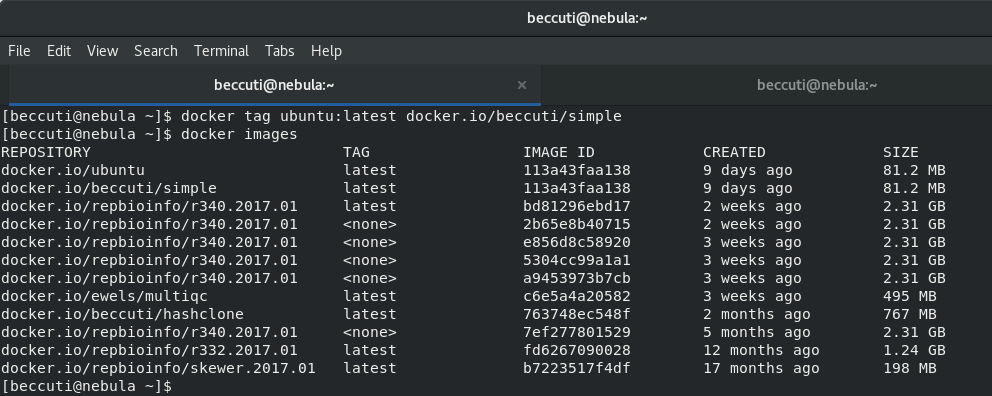
\includegraphics[width=1.0\columnwidth]{./Figure/tag}
  		\end{center}
} 
  	
  	
 	     \frame{
\frametitle{Building a Docker Image} 
  
 \emph{\color{PineGreen} docker run -it $\langle \it{target\_image} \rangle$ /bin/bash} can be used to run a specific docker image interactively.
     	\begin{center}
  			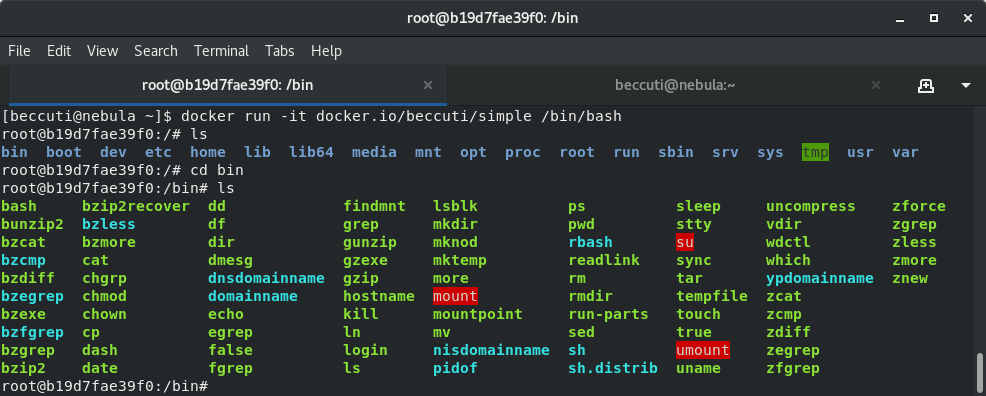
\includegraphics[width=1.00\columnwidth]{./Figure/run}
  		\end{center}  
  
 }  	
  	
\frame{
\frametitle{Building a Docker Images} 
  
Commands can be executed on a container as a remote machine.   \vspace{0.2cm}
     	\begin{center}
  			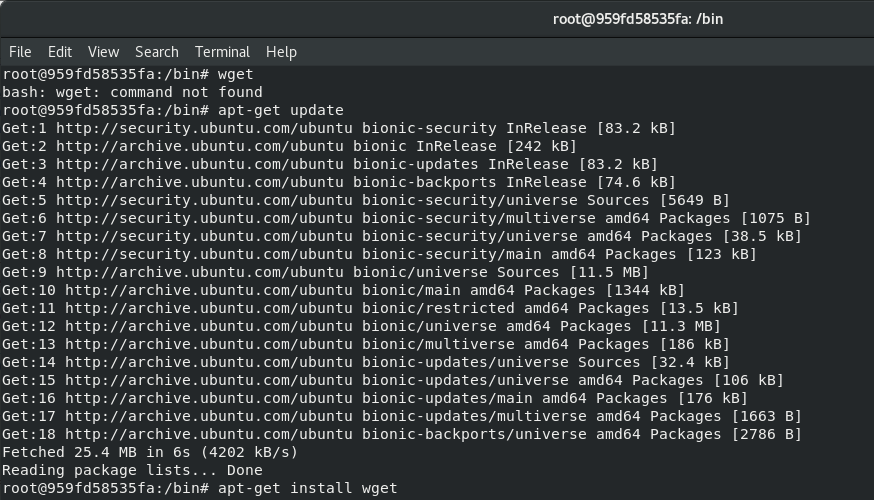
\includegraphics[width=1.00\columnwidth]{./Figure/run2}
  		\end{center}  
  
 }
 
 
    	     \frame{
\frametitle{Building a Docker Image} 
 
 \emph{\color{PineGreen} docker ps -a} can be used  to list the running and executed containers.\vspace{0.2cm}
     	\begin{center}
  			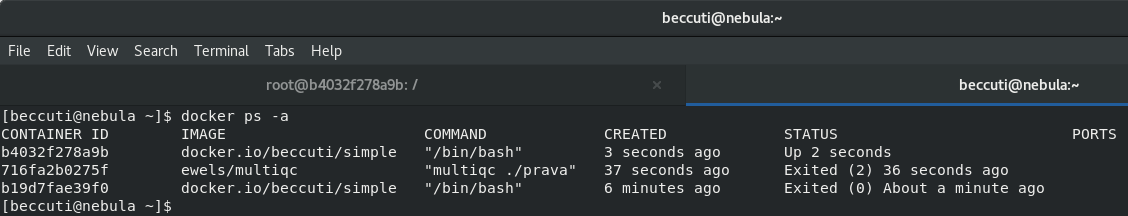
\includegraphics[width=1.01\columnwidth]{./Figure/ps}
  		\end{center}  
  
 }
 
 
  
    	     \frame{
\frametitle{Building a Docker Image} 
 
 \emph{\color{PineGreen} docker ps  -f $\langle \it{filter\_cond} \rangle$} lists only the containers satisfying filter condition.
%     	\begin{center}
 % 			\includegraphics[width=1.00\columnwidth]{./Figure/%ps1}
  %		\end{center}  
       	\begin{center}
  			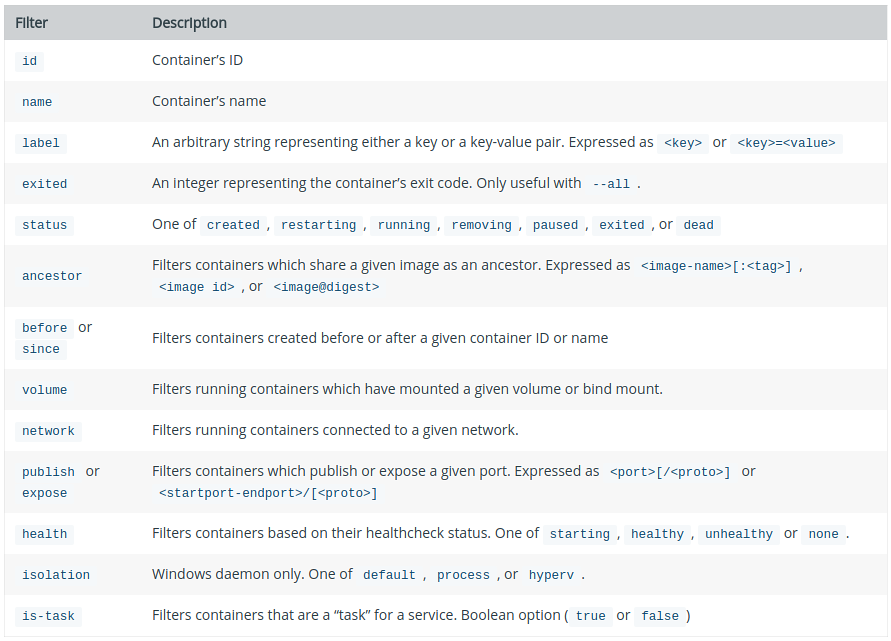
\includegraphics[width=0.90\columnwidth]{./Figure/filter}
  		\end{center}  
 }
     	     \frame{
\frametitle{Building a Docker Image} 
 
 \emph{\color{PineGreen} docker ps -f $\langle \it{filter\_cond} \rangle$} lists only the containers satisfying filter condition.
    	\begin{center}
  			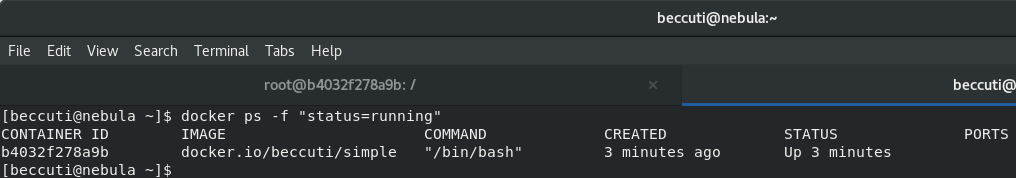
\includegraphics[width=1.00\columnwidth]{./Figure/ps1}
  		\end{center}  
  %     	\begin{center}
  %			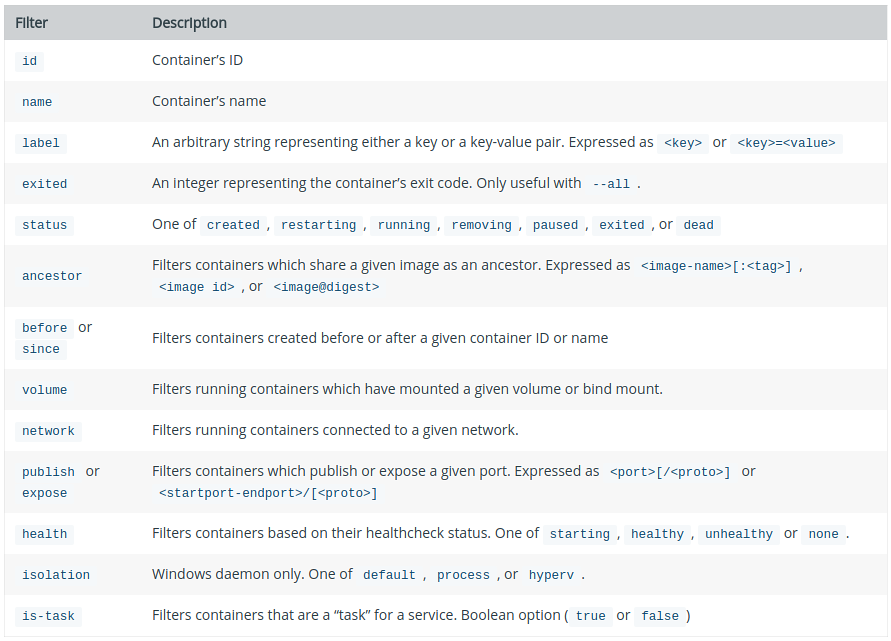
\includegraphics[width=0.90\columnwidth]{./Figure/filter}
  %		\end{center}  
 }
 
 
 
 
 \frame{
\frametitle{Building a Docker Image} 
A commit must be executed to make permanent the image update. \\\vspace{0.1cm}
 \emph{\color{PineGreen} docker commit [ContainerID] [Repository[:Tag]} commits the container image \vspace{0.1cm}
 	     	\begin{center}
  			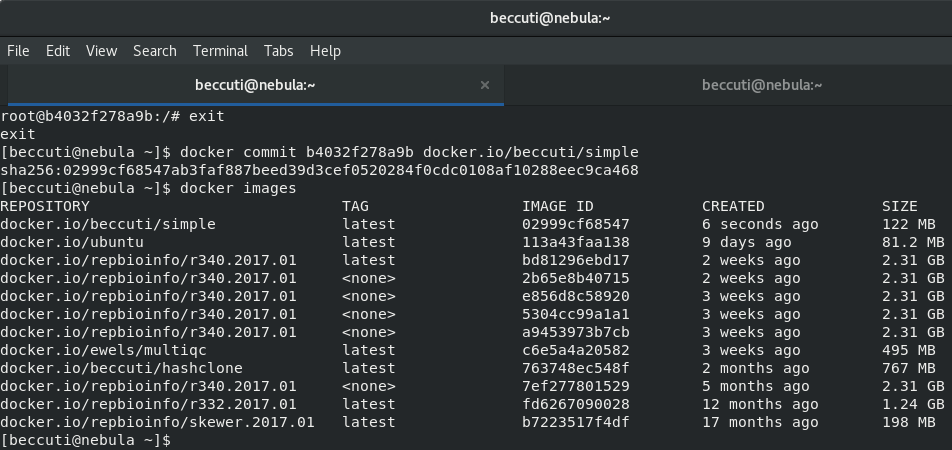
\includegraphics[width=1.0\columnwidth]{./Figure/commit}
  		\end{center}  
 	}
  	
  	
  	
       \frame{
\frametitle{Building a Docker Image} 
  
 \emph{\color{PineGreen} docker push 
 $\langle \it{image} \rangle$} can be used to upload a docker image into  a hub.
     	\begin{center}
  			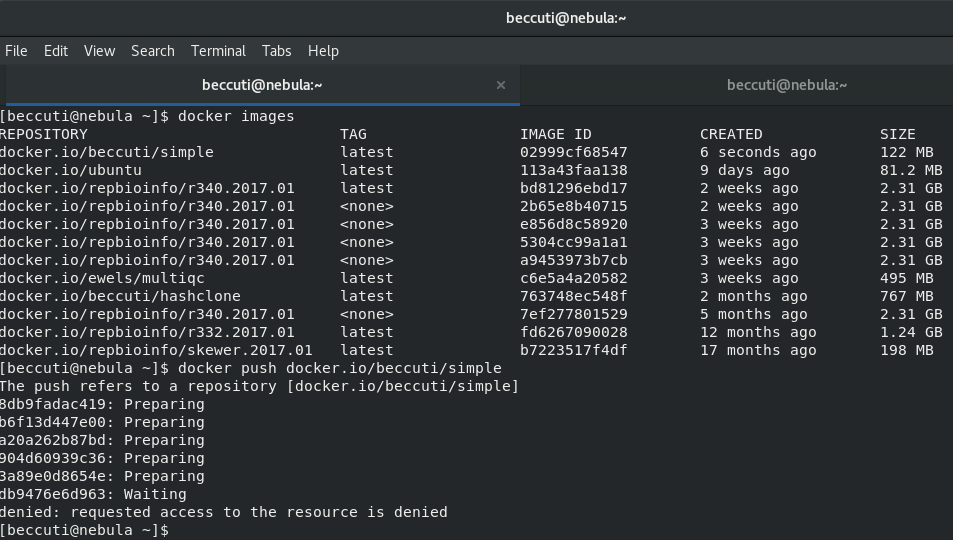
\includegraphics[width=1.00\columnwidth]{./Figure/push}
  		\end{center}  
  
  \vspace{0.2cm}
 \centerline{\textbf{\color{NavyBlue}User  must be logged into the repository}}	
 }	
 
        \frame{
\frametitle{Building a Docker Image} 
  
 \emph{\color{PineGreen} docker login}  can be exploited to login into the repository.
     	\begin{center}
  			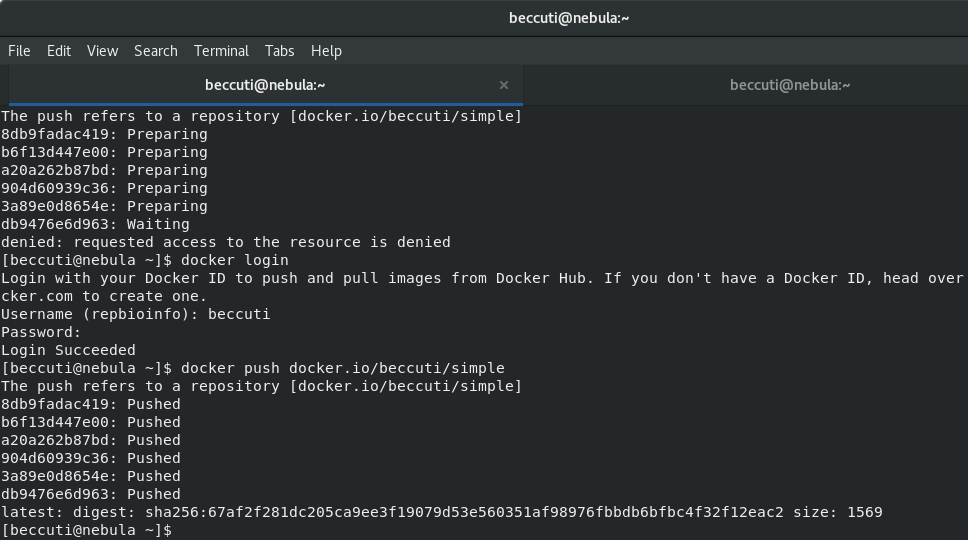
\includegraphics[width=1.00\columnwidth]{./Figure/login1}
  		\end{center}  
 }	
  	
  	
  	      \frame{
\frametitle{Building a Docker Image} 
  
 \emph{\color{PineGreen} docker push 
 $\langle \it{image} \rangle$} can be used to upload a docker image into  a hub.
     	\begin{center}
  			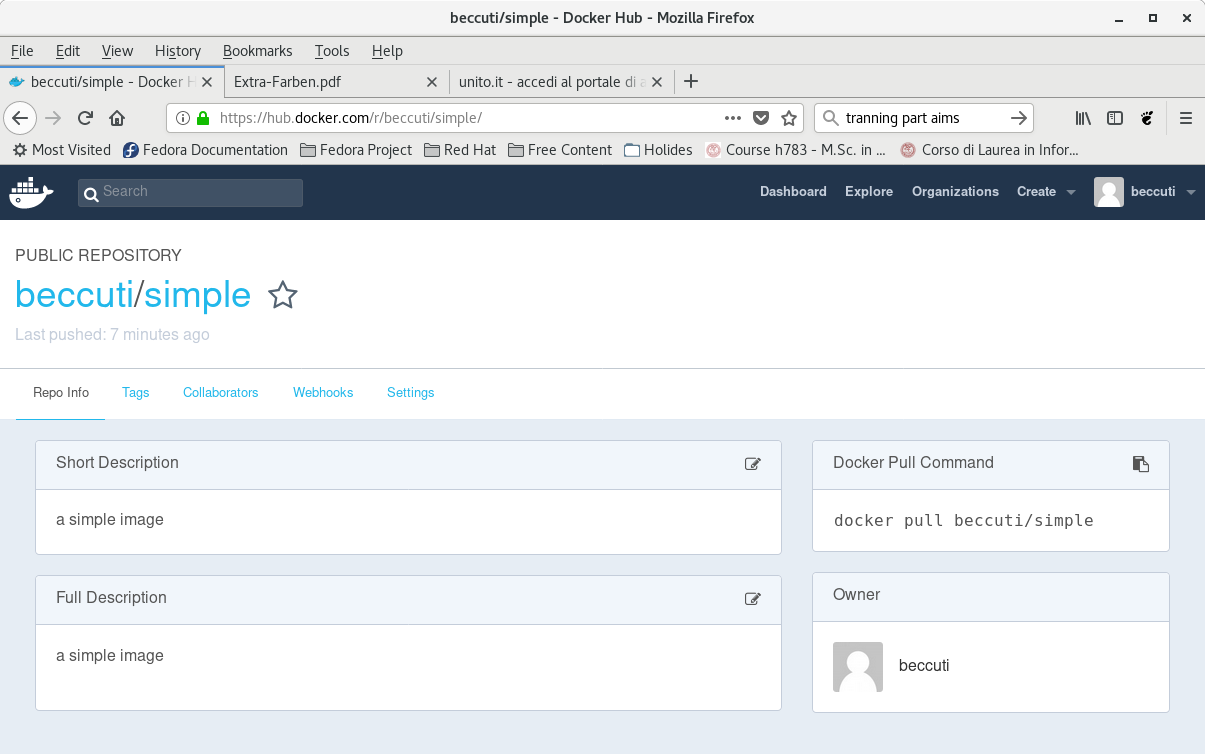
\includegraphics[width=0.90\columnwidth]{./Figure/push2}
  		\end{center}  
  
 } 	
  		 
  		 
  		 
        \frame{
\frametitle{Building a Docker Image with R} 

Install R environment in the docker image previously created.
 		     	\begin{center}
  			
\includegraphics[width=1.00\columnwidth]{./Figure/installR}
  		\end{center}  
\vspace{0.2cm} Update our docker image.
  		
 		     	\begin{center}
  			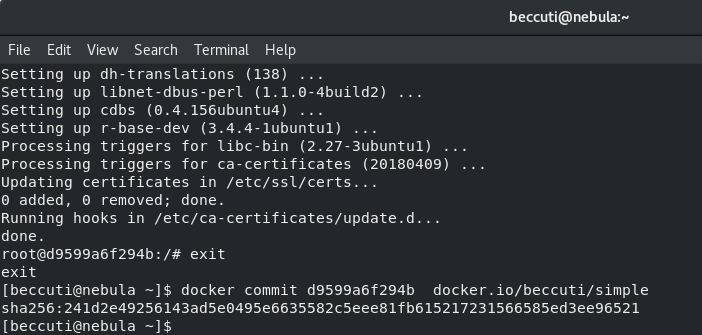
\includegraphics[width=1.00\columnwidth]{./Figure/commit3}
  		\end{center}    		
 } 	  		 
  
 
 
  		 
        \frame{
\frametitle{Building a Docker Image with R} 

A Docker image with R base is already available 
 		     	\begin{center}
  			\includegraphics[width=1.00\columnwidth]{./Figure/installRbase}
  		\end{center} 
 }
 
 
         \frame{
\frametitle{Building a Docker Image with R} 

Comparing image dimensions:
 		     	\begin{center}
  			\includegraphics[width=1.00\columnwidth]{./Figure/installRbase2}
  		\end{center} 
 }
  
  
    \frame{
  \frametitle {Our first simple Docker image}
 To create this image we will perform the following tasks:\vspace{0.4cm}
 \begin{itemize}
 \item Create an own docker public repository;\vspace{0.2cm}
 \item Download a  base image from the Docker Hub;\vspace{0.2cm}	
 \item Updating the download image and upload it on our own repository;\vspace{0.2cm}	
 \item Create and embed  simple BASH and R  scripts on our image;\vspace{0.2cm}	
 \item Execute the new created image.
 \end{itemize}
} 
   
  
         \frame{
\frametitle{Our first simple Docker image} 

\textbf{\color{NavyBlue}Create R and Bash scripts.}
\begin{itemize}
\item We use \textbf{\color{NavyBlue}Rstudio} to create our  R script; %\vspace{-0.1cm}
 \begin{center}
  			\includegraphics[width=0.93\columnwidth]{./Figure/rscript}
 \end{center} \vspace{-0.1cm}
It takes as input two vectors x and y returns their sum and difference. 
 \end{itemize}
 } 	  		 
  	
  		 
\frame{
\frametitle{Our first simple Docker image} 

\textbf{\color{NavyBlue}Create R and Bash scripts.}\vspace{0.1cm}
\begin{itemize}
\item We use \textbf{\color{NavyBlue}gedit} to create our Bash script; \vspace{0.2cm}
 \begin{center}
  			\includegraphics[width=0.93\columnwidth]{./Figure/shscript}
 \end{center} \vspace{0.2cm}
 It takes as input the two values and calls the R script previously created. 
 \end{itemize}
 } 	
 

   	  
         \frame{
\frametitle{Our first simple Docker image} \vspace{0.3cm}
Copy the two scripts in the docker image \vspace{0.2cm}
 		     	\begin{center}
  			\includegraphics[width=1.00\columnwidth]{./Figure/run3}
  		\end{center}  	
 	   	  
\begin{itemize}
\item  Option \emph{\color{PineGreen}-v} is used to mount a local folder  as a volume into the container;\vspace{0.2cm}
\item If you cannot access the volume in the container then the security level  of your machine could be too stringent;\vspace{0.2cm}
\item Option  \emph{\color{PineGreen} -\;-privileged=true} can be exploited to cope with this.
\end{itemize}
   

}	  
  
       \frame{
\frametitle{Our first simple Docker image} \vspace{0.3cm}
Copy the two scripts in the docker image \vspace{0.2cm}
 		     	\begin{center}
  			\includegraphics[width=1.00\columnwidth]{./Figure/run5}
  		\end{center}  	
  		}
  
  
  

 	
 	
 	          \frame{
\frametitle{Our first simple Docker image} 
To execute the script passing two input parameters
 		     	\begin{center}
  			\includegraphics[width=0.80\columnwidth]{./Figure/run4}
  		\end{center}  	
 } 	
 
 
 
  \frame{
\frametitle{Our first simple Docker image} 
\begin{columns}[T] % align columns
  \begin{column}{.26\textwidth}
  \vspace{4cm}
   \hspace{0.25cm}Expected output of\\ 
     \hspace{0.25cm}our script: 
   \end{column}%
   \hfill%
   \begin{column}{0.85\textwidth}
   \vspace{-0.3cm}
    \begin{center}
  			\includegraphics[width=0.70\columnwidth]{./Figure/shscript1}
 \end{center}
      \end{column}%
   \end{columns}

 } 	
   	  



\frame{
\frametitle {}
\vspace{2cm}
\centerline{\Huge \color{NavyBlue} \textbf{\emph{Dockerfile}}}
\vspace{0.5cm}
}
\begin{frame}
\frametitle{Dockefile}

A docker can be created by hand

\begin{itemize}
\item pull an image
\item star a container
\item modify the container
\item commit the changes 
\end{itemize}

this is more or less the process for creating a reusable container \textit{an Image}
\end{frame}

\begin{frame}
\frametitle{Dockerfile}

By \textit{hand} is good for practicing or testing but is very bad for 
\begin{itemize}
\item reproducibility
\item automation
\item dependencies
\end{itemize}
\end{frame}

\begin{frame}
\frametitle{Dockerfile}

By \textit{hand} is good for practicing or testing but is very bad for 

\begin{itemize}
\item \textit{reproducibility}: lost the history of the commands that create the final image
\item automation
\item dependencies
\end{itemize}
\end{frame}

\begin{frame}
\frametitle{Dockerfile}

By \textit{hand} is good for practicing or testing but is very bad for 

\begin{itemize}
\item reproducibility
\item \textit{automation}: images are lost because some disaster and eveything was on a local machine
\item dependencies
\end{itemize}
\end{frame}

\begin{frame}
\frametitle{Dockerfile}

By \textit{hand} is good for practicing or testing but is very bad for 

\begin{itemize}
\item reproducibility
\item automation
\item \textit{dependencies}: images are build from other images and something must be changed in the original image
\end{itemize}
\end{frame}

\begin{frame}
\frametitle{Dockerfile}
\framesubtitle{what is it?}

A simple text files with all the instructions for

\begin{itemize}
\item start (PULL) from a (public) Linux distribution
\item install software
\item configure the installation
\item configure the container for running automatically
\end{itemize}
\end{frame}

\begin{frame}[fragile]
\frametitle{Dockerfile}
\framesubtitle{what is it?}

The most minimal \lstinline!Dockerfile!
\begin{lstlisting}
FROM ubuntu:18.04
\end{lstlisting}

\textit{Note} by convention \lstinline!Dockerfile! is the name to use for the file containing the instructions.
\end{frame}


\begin{frame}[fragile]
\frametitle{Dockerfile}
\framesubtitle{How to use it}

A \lstinline!Dockerfile! can be used for building a new image

\begin{lstlisting}
 $ docker build -t origin .
 Sending build context to Docker daemon  2.048kB
 Step 1/1 : FROM ubuntu:18.04
  ---> cd6d8154f1e1
  Successfully built cd6d8154f1e1
  Successfully tagged origin:latest
\end{lstlisting}

A new image is created with the \lstinline!sha256! \lstinline!cd6d8154f1e1! called \lstinline!origin! and the version, in this case by default \lstinline!Docker! assign the tag \lstinline!latest!
\end{frame}

\begin{frame}[fragile]
\frametitle{Dockerfile}
\framesubtitle{FROM}

Start from a Linux distribution or previous installations/images

\begin{lstlisting}
FROM <image> [AS <name>]

FROM <image>[:<tag>] [AS <name>]

FROM <image>[@<digest>] [AS <name>]
\end{lstlisting}
\end{frame}

\begin{frame}[fragile]
\frametitle{Dockerfile}
\framesubtitle{LABEL}

Metadata are useful in order to describe the image, making it more consumable by others

\lstinline!LABEL <key>=<value> <key>=<value> <key>=<value> ...!

\begin{lstlisting}
LABEL org.ingm.group="Your Boss name"
LABEL maintainer="Bonnal Raoul J.P. <bonnal@ingm.org>"
LABEL project="Elixir Test"
LABEL description="Dockerfile example \
with multiple lines."
LABEL version="1.2"
 
LABEL maintainer=''bonnal@ingm.org''
\end{lstlisting}

User is free to use any kind of \lstinline!key=val! convention but the \textit{reverse DNS} notation.
\end{frame}

\begin{frame}[fragile]
\frametitle{Dockerfile}
\framesubtitle{ENV}

Environment variables can be set inside the container

\begin{lstlisting}
ENV <key> <value>
ENV <key>=<value> ...
\end{lstlisting}

\begin{lstlisting}[breaklines=true]
ENV software="samtools" description=A\ great\ piece\ of\ software
    author=someone
\end{lstlisting}	
and
	
\begin{lstlisting}
ENV software samtools
ENV description A great piece of software
ENV author someone
\end{lstlisting}

these variable are available during the building process and when the container is running
\end{frame}

\begin{frame}[fragile]
\frametitle{Dockerfile}
\framesubtitle{WORKDIR}

Sets the working directory for the following \textit{instructions}

\begin{lstlisting}
ENV MYSUBDIR mytmp
RUN mkdir /opt/$MYSUBDIR
WORKDIR /opt/$MYSUBDIR
RUN pwd
\end{lstlisting}

Works for \lstinline!RUN!, \lstinline!CMD!, \lstinline!ENTRYPOINT!, \lstinline!COPY! and \lstinline!ADD!
\end{frame}

\begin{frame}[fragile]
\frametitle{Dockerfile}
\framesubtitle{injecting files}

To fully customize the image, external files can be included. To achieve this \textit{Docker} provides two different tools

\begin{itemize}
\item \lstinline!ADD!
\item \lstinline!COPY!
\end{itemize}
\end{frame}

\begin{frame}[fragile]
\frametitle{Dockerfile}
\framesubtitle{ADD}

\begin{lstlisting}
ADD [--chown=<user>:<group>] <src>... <dest>
ADD [--chown=<user>:<group>] ["<src>",... "<dest>"]
\end{lstlisting}
\begin{itemize}
\item Digest URLs, download
\item Unpack archives (identity, gzip, bzip2 or xz)
\item Does not perform authentication
\item At every build it is re excuted
\end{itemize}
\end{frame}

\begin{frame}[fragile]
\frametitle{Dockerfile}
\framesubtitle{COPY}

\begin{lstlisting}
COPY [--chown=<user>:<group>] <src>... <dest>
COPY [--chown=<user>:<group>] ["<src>",... "<dest>"]
\end{lstlisting}

\begin{itemize}
\item Relative path outside of context does not work
\item Works only with local files or directory
\item Can copy files from source location to a previous build stage \lstinline!FROM!
\item NO URLs
\item NO auto unpacking
\end{itemize}
\end{frame}

\begin{frame}[fragile]
\frametitle{Dockerfile}
\framesubtitle{SHELL}

When commands must be run with a different shell

\begin{lstlisting}
SHELL ["executable", "parameters"]
\end{lstlisting}
\end{frame}

\begin{frame}[fragile]
\frametitle{Dockerfile}
\framesubtitle{USER}

Set the USER to use during when the containers run.
It also set the user for \lstinline!RUN!, \lstinline!CMD!, \lstinline!ENTRYPOINT! following the declaration of \lstinline!USER!

\begin{lstlisting}
USER <user>[:<group>]
USER <UID>[:<GID>]
\end{lstlisting}
\end{frame}

\begin{frame}[fragile]
\frametitle{Dockerfile}
\framesubtitle{RUN}

To customise the installation the user must execute commands.

The commands are run inside a default shell \lstinline!/bin/sh -c!

Use the \lstinline!SHELL! clause to change the shell for the following \lstinline!Dockerfile!

When a \lstinline!RUN! succeed Docker will write a layer.
\end{frame}

\begin{frame}[fragile]
\frametitle{Dockerfile}
\framesubtitle{RUN}

\lstinline!RUN! have two forms:

\begin{lstlisting}
RUN apt-get update
\end{lstlisting}

or use a more explicit form where parameters are passed in a sort of \lstinline!JSON! notation

\begin{lstlisting}
RUN ["apt-get", "update"]
\end{lstlisting}

The JSON form does not create a shell for the command, so variable can not be substituted. To use the shell substitution call the shell first.
\end{frame}

\begin{frame}[fragile]
\frametitle{Dockerfile}
\framesubtitle{RUN}

\begin{lstlisting}
RUN apt-get install -y wget git python3.6
\end{lstlisting}

A \lstinline!RUN! command can span multiple lines


\begin{lstlisting}
RUN apt-get install -y wget \
                       git \
				  python3.6
\end{lstlisting}
\end{frame}

\begin{frame}[fragile]
\frametitle{Dockerfile}
\framesubtitle{RUN}

A \lstinline!RUN! command can be made by multiple commands

\begin{lstlisting}
RUN comamnd1 && command2
\end{lstlisting}

The \lstinline!RUN! will pass and create a layer only if it succeed. Otherwise, Docker will report the original error.
\end{frame}

\begin{frame}[fragile]
\frametitle{Dockerfile}
\framesubtitle{RUN}

Combining commands and spanning the commands on multiple lines helps in readability and building complex configurations.

\begin{lstlisting}
RUN apt-get update &&\
    apt-get install -y wget 
\end{lstlisting}
\end{frame}

\begin{frame}[fragile]
\frametitle{Dockerfile}
\framesubtitle{RUN}

Combining commands and spanning the commands on multiple lines helps in readability and building complex configurations.

\begin{lstlisting}
RUN apt-get update &&\
    apt-get install -y wget \
	                   git \
	                   python3.6
\end{lstlisting}
\end{frame}

\begin{frame}[fragile]
\frametitle{Dockerfile}
\framesubtitle{ENTRYPOINT}
Defines a container that runs as an executable

Forms:

\begin{itemize}
\item \textit{exec}: preferred \lstinline!ENTRYPOINT ["executable", "param1", "param2"]!

\item \textit{shell}:  \lstinline!ENTRYPOINT command param1 param2!
\end{itemize}
\end{frame}


\begin{frame}[fragile]
\frametitle{Dockerfile}
\framesubtitle{CMD}
Defines the default behavior for the container.

Forms:
\begin{itemize}
\item \textit{exec}: preferred \lstinline!CMD ["executable","param1","param2"]!
\item default parameters to \lstinline!ENTRYPOINT!: \lstinline!CMD ["param1","param2"]!
\item \textit{shell}: \lstinline!CMD command param1 param2!
\end{itemize}
\end{frame}

\begin{frame}[fragile]
\frametitle{Dockerfile}
\framesubtitle{VOLUME}
It is possible to embed the volume definition at build time.

Any change, at build time, after the definition will be discarded.

\begin{lstlisting}
VOLUME ["/path","..."]

VOLUME /path_a /path_b
\end{lstlisting}

Volumes are:
\begin{itemize}
\item created automatically at run time
\item can be shared between containers with \lstinline!--volumes-from!
\item are anonymous at runtime
\item can be inspected looking at \lstinline!/var/lib/docker/volumes!
\end{itemize}
\end{frame}

\begin{frame}[fragile]
\frametitle{Dockerfile}
\framesubtitle{VOLUME}

Example of creating a \lstinline!VOLUME!

\begin{lstlisting}[breaklines=true]
FROM ubuntu:18.04
RUN mkdir /opt/elixir-volume
RUN echo "This is a file with a foo text" > /opt/elixir-volume/README.txt
VOLUME ["/opt/elixir-volume"]
\end{lstlisting}
\end{frame}

\begin{frame}[fragile]
\frametitle{Dockerfile}
\framesubtitle{context}

Context defines what is visible at the build time by Docker.
Data inside the \textit{context} are copied in a temporary place where the building process is working. The building process can see only data in that temporary place. 

This process of \textit{building the context} can take a lot of time if files are big and many.

Avoid:
\begin{itemize}
\item huge files
\item temporary or working file
\item backup 
\end{itemize}

in the context.

A lean \textit{context} means quick build.
\end{frame}

\begin{frame}
\frametitle{Dockerfile}
\framesubtitle{validation}

A \textit{Dockerfile} is a text file and Docker keep tracks of changes in the file.

Most of the \textit{instructions} generate a layer. 

Changes to the text are invalidaing all the following \textit{instructions} and they will be re-executed.
\end{frame}

\begin{frame}[fragile]
\frametitle{Dockerfile}
\framesubtitle{example}

\begin{lstlisting}
FROM ubuntu:18.04

LABEL org.ingm.group="Your Boss name"
LABEL maintainer="Bonnal Raoul J.P. <bonnal@ingm.org>"
LABEL project="Elixir Test"
LABEL description="Dockerfile example"
LABEL version="1.2"

RUN apt-get update &&\
    apt-get install -y wget \
	                   git \
	                   python3.6
\end{lstlisting}
\end{frame}

\begin{frame}[fragile]
\frametitle{Dockerfile}
\framesubtitle{bulding}

\begin{lstlisting}
$ docker build -t origin .

$ docker build -t origin Dockerfile .

$ docker build -t origin -f /absolute/path/Dockerfile .
\end{lstlisting}
\end{frame}

\begin{frame}
\frametitle{Dockerfile}
\framesubtitle{building}

\includegraphics[width=0.8\columnwidth]{./Figure/BuildingDockerfile}
\end{frame}



 	
 \frame{
  \frametitle {}
  \vspace{1cm}
  \centerline{\Huge \color{NavyBlue} \textbf{\emph{Our first simple Docker image}}}
   \centerline{\Huge \color{NavyBlue} \textbf{\emph{using dockerfile}}}
   		     	\begin{center}
  			\includegraphics[width=0.60\columnwidth]{./Figure/dockerfile}
  		\end{center}   
   
}



  
  \frame{
  \frametitle{Dockerfile in a nutshell} 
  \begin{itemize}
  \item  Docker images can be built automatically by reading the instructions from a \textbf{\color{NavyBlue}Docker file};\vspace{0.2cm}
  \item  Docker file is a \textbf{\color{NavyBlue}simple text file} with the instructions on how to build your images;\vspace{0.2cm}
  \item The main Dockerfile commands are:\vspace{0.1cm}
  \begin{description}
  \item[FROM] It defines the base image to use  for the build process;
  \item[RUN]  It takes a command as its argument and runs it to form the image; 
  \item[COPY] It copies files from the source on the host into the container filesystem;
  \item[CMD]  It specifies what command to run within the container.  
  \end{description}
  \end{itemize}
  }
  
  
      \frame{
  \frametitle {Our first simple Docker image using dockerfile}
 This requires the following tasks:\vspace{0.4cm}
 \begin{itemize}
 \item Create a dockerfile;\vspace{0.2cm}	
 \item Create the images using the generated dockerfile.
 \end{itemize}
} 
  
        \frame{
  \frametitle {Our first simple Docker image using dockerfile}
 This requires the following tasks:\vspace{0.4cm}
 \begin{itemize}
 \item Create a dockerfile;\vspace{0.2cm}	\color{grey}
 \item Create the images using the generated dockerfile.
 \end{itemize}
} 
  
          \frame{
  \frametitle {Create a dockerfile}
  We use \textbf{\color{NavyBlue}gedit} to create our dockerfile; \vspace{0.2cm}
 \begin{center}
  			\includegraphics[width=0.93\columnwidth]{./Figure/gedit}
 \end{center} 
  }
   	  	
       \frame{
  \frametitle {Our first simple Docker image using dockerfile}
 This requires the following tasks:\vspace{0.4cm}
 \begin{itemize}
 \item Create a dockerfile;\vspace{0.2cm}	
 \item Create the images using the generated dockerfile.
 \end{itemize}
}   	  	


  	      \frame{
\frametitle{Building a Docker Image} 
  
 \emph{\color{PineGreen} docker build -t  $\langle \it{image} \rangle$ $\langle \it{path} \rangle$} can be used to build an image from a Dockerfile.
     	\begin{center}
  			\includegraphics[width=1.00\columnwidth]{./Figure/build}
  		\end{center}  
  		     	\begin{center}
  			\includegraphics[width=1.00\columnwidth]{./Figure/build1}
  		\end{center}  
  
 }

\frame{
\frametitle {}
\vspace{2cm}
\centerline{\Huge \color{NavyBlue} \textbf{\emph{Dockerfile Best Practices}}}
\vspace{0.5cm}
}

\begin{frame}[fragile]
\frametitle{Dockerfile}
\framesubtitle{from \lstinline!stdin!}

Building an image on the fly, w/o using a static file

\begin{lstlisting}
touch myfile.sh
chmod +x myfile.sh
docker build -t foo . -f-<<EOF
FROM ubuntu:18.04
RUN echo "hello world"
COPY myfile.sh /opt/
EOF
\end{lstlisting}
\end{frame}


\begin{frame}[fragile]
\frametitle{Dockerfile}
\framesubtitle{with a remote context}

\begin{lstlisting}
docker build -t foo \
       https://github.com/thajeztah/pgadmin4-docker.git \
	   -f-<<EOF
	   FROM ubuntu:18.04
	   WORKDIR /usr/local/lib/python2.7/site-packages
	   COPY LICENSE pgadmin4/
	   COPY config_distro.py pgadmin4/
	   EOF
\end{lstlisting}
\end{frame}

\begin{frame}[fragile]
\frametitle{Dockerfile}
\framesubtitle{ignore files}

Unwanted files can be excluded from the context, by convention
a \lstinline!.dockerignore! file is required and using regular expression
is possible to exclude files.
\end{frame}

\begin{frame}[fragile]
\frametitle{Dockerfile}
\framesubtitle{ignore files}

\begin{itemize}
\item \lstinline!#!: defines a comment
\item \lstinline!*/temp*! Exclude files and directories whose names start with temp in any immediate subdirectory of the root.For example, the plain file \lstinline!/somedir/temporary.txt! is excluded, as is the directory \lstinline!/somedir/temp!.
\item \lstinline!|*/*/temp*! Exclude files and directories starting with temp from any sub-directory that is two levels below the root. For example, \lstinline!/somedir/subdir/temporary.txt! is excluded.
\item \lstinline!temp?! Exclude files and directories in the root directory whose names are a one-character extension of temp. For example, \lstinline!/tempa! and \lstinline!/tempb! are excluded.
\end{itemize}
\end{frame}

\begin{frame}[fragile]
\frametitle{Dockerfile}
\framesubtitle{make it human readable}

When possible sorting multi-line arguments is recommended

\begin{lstlisting}
RUN apt-get update &&\
    apt-get install -y \
	    bzr \
		csv \
		git \
		mercurial \
		subversion \
		texlive
\end{lstlisting}
\end{frame}


\begin{frame}[fragile]
\frametitle{Dockerfile}
\framesubtitle{quick tips}

\begin{itemize}
\item Annotate the image with \lstinline!LABEL!
\item Use \lstinline!ENV! for keeping track of versions
\item \lstinline!COPY! is more transparent than \lstinline!ADD!
\item Use \lstinline!wget! or \lstinline!curl! for downloading from the web
\item The web does not guarantee URLs forever
  \begin{itemize}
  \item Consider to host a web/fileserver for \textit{very important} data or software
  \item Licensing can be an issue, some software can not be distributed freely
  \end{itemize}
\item Use \lstinline!WORKDIR! when possible
\item Image as executable ? \lstinline!ENTRYPOINT! is the way to go
  \begin{itemize}
  \item \lstinline!CMD! is used for default parameters \lstinline!--help!
  \end{itemize}
\item A regular user with \lstinline!root! privileges is worst than evil
  \begin{itemize}
  \item This applies only if it is your infrastructure \lstinline!:)!
  \item In most scientific infrastructures Docker is forbidden or masked by some wrapper
  \end{itemize}
\end{itemize}
\end{frame}
 

  	
   	  		 
 \end{document}  

  

